\chapter{Machin Learning Results}
\section{Datasets informations}


            \begin{longtable}{|c|c|c|c|}
            \caption{Datasets used in the experiments}\label{annexes:datasets_descriptions} \\
            \hline
            \textbf{Dataset Number} & \textbf{Dataset Name} & \textbf{Filter Entropy} & \textbf{Filter Chunk Size} \\
            \hline
            \endfirsthead
            \multicolumn{4}{c}
            {\tablename\ \thetable\ -- continued from previous page} \\
            \hline
            \textbf{Dataset Number} & \textbf{Dataset Name} & \textbf{Filter Entropy} & \textbf{Filter Chunk Size} \\
            \hline
            \endhead
            \hline \multicolumn{4}{|r|}{Continued on next page} \\ \hline
            \endfoot
            \hline
            \endlastfoot
            24 & chunk\_extraction & False & False \\
\hline
25 & chunk\_extraction & False & True \\
\hline
26 & chunk\_extraction & True & False \\
\hline
27 & chunk\_extraction & True & True \\
\hline
\end{longtable}

\section{Timeout instances}

\label{sec:annexe:timeout_instances}

\begin{table}[ht]
\centering
\begin{tabular}{ll}
\hline
dataset & instance \\ 
\hline
25 chunk\_extraction (filtered chunk size) & Transformers 0 \\ 
25 chunk\_extraction (filtered chunk size) & Transformers 1 \\ 
26 chunk\_extraction (filtered entropy) & Transformers 2 \\ 
26 chunk\_extraction (filtered entropy) & Transformers 3 \\ 
26 chunk\_extraction (filtered entropy) & Transformers 4 \\ 
26 chunk\_extraction (filtered entropy) & Transformers 5 \\ 
26 chunk\_extraction (filtered entropy) & Transformers 6 \\ 
26 chunk\_extraction (filtered entropy) & Transformers 7 \\ 
\hline
\end{tabular}
\caption{Timeouts instances}
\label{tab:timeouts}
\end{table}

\section{Feature engineering fails}

\label{sec:annexe:feature_engineering_fails}

The list is empty.

\section{Out of memory instances (Classifications)}

\label{sec:annexe:out_of_memory_instances_classifications}

\begin{table}[ht]
\centering
\begin{tabular}{ll}
\hline
dataset & instance \\ 
\hline
24 chunk\_extraction & Transformers 0 \\ 
24 chunk\_extraction & Transformers 1 \\ 
24 chunk\_extraction & Transformers 2 \\ 
24 chunk\_extraction & Transformers 3 \\ 
24 chunk\_extraction & Transformers 4 \\ 
24 chunk\_extraction & Transformers 5 \\ 
24 chunk\_extraction & Transformers 6 \\ 
24 chunk\_extraction & Transformers 7 \\ 
24 chunk\_extraction & Word2vec 0 \\ 
24 chunk\_extraction & Word2vec 1 \\ 
24 chunk\_extraction & Word2vec 2 \\ 
24 chunk\_extraction & Word2vec 3 \\ 
24 chunk\_extraction & Word2vec 4 \\ 
24 chunk\_extraction & Word2vec 5 \\ 
24 chunk\_extraction & Word2vec 6 \\ 
24 chunk\_extraction & Word2vec 7 \\ 
24 chunk\_extraction & Word2vec 8 \\ 
24 chunk\_extraction & Word2vec 9 \\ 
24 chunk\_extraction & Word2vec 10 \\ 
24 chunk\_extraction & Word2vec 11 \\ 
25 chunk\_extraction (filtered chunk size) & Transformers 2 \\ 
25 chunk\_extraction (filtered chunk size) & Transformers 3 \\ 
25 chunk\_extraction (filtered chunk size) & Transformers 4 \\ 
25 chunk\_extraction (filtered chunk size) & Transformers 5 \\ 
25 chunk\_extraction (filtered chunk size) & Transformers 6 \\ 
25 chunk\_extraction (filtered chunk size) & Transformers 7 \\ 
25 chunk\_extraction (filtered chunk size) & Word2vec 10 \\ 
25 chunk\_extraction (filtered chunk size) & Word2vec 11 \\ 
\hline
\end{tabular}
\caption{Out of memory instances (Classifications)}
\label{tab:annexe:out_of_memory_instances_classifications}
\end{table}

\section{Out of memory instances (Clustering)}

\label{sec:annexe:out_of_memory_instances_clustering}

\begin{table}[ht]
\centering
\begin{tabular}{ll}
\hline
dataset & instance \\ 
\hline
24 chunk\_extraction & Transformers 0 \\ 
24 chunk\_extraction & Transformers 1 \\ 
24 chunk\_extraction & Transformers 2 \\ 
24 chunk\_extraction & Transformers 3 \\ 
24 chunk\_extraction & Transformers 4 \\ 
24 chunk\_extraction & Transformers 5 \\ 
24 chunk\_extraction & Transformers 6 \\ 
24 chunk\_extraction & Transformers 7 \\ 
24 chunk\_extraction & Word2vec 0 \\ 
24 chunk\_extraction & Word2vec 1 \\ 
24 chunk\_extraction & Word2vec 2 \\ 
24 chunk\_extraction & Word2vec 3 \\ 
24 chunk\_extraction & Word2vec 4 \\ 
24 chunk\_extraction & Word2vec 5 \\ 
24 chunk\_extraction & Word2vec 6 \\ 
24 chunk\_extraction & Word2vec 7 \\ 
24 chunk\_extraction & Word2vec 8 \\ 
24 chunk\_extraction & Word2vec 9 \\ 
24 chunk\_extraction & Word2vec 10 \\ 
24 chunk\_extraction & Word2vec 11 \\ 
25 chunk\_extraction (filtered chunk size) & Transformers 2 \\ 
25 chunk\_extraction (filtered chunk size) & Transformers 3 \\ 
25 chunk\_extraction (filtered chunk size) & Transformers 4 \\ 
25 chunk\_extraction (filtered chunk size) & Transformers 5 \\ 
25 chunk\_extraction (filtered chunk size) & Transformers 6 \\ 
25 chunk\_extraction (filtered chunk size) & Transformers 7 \\ 
25 chunk\_extraction (filtered chunk size) & Word2vec 10 \\ 
25 chunk\_extraction (filtered chunk size) & Word2vec 11 \\ 
\hline
\end{tabular}
\caption{Out of memory instances (Clustering)}
\label{tab:annexe:out_of_memory_instances_clustering}
\end{table}

\section{Feature Engineering results}

\label{sec:annexe:feature_engineering_results}

\subsection{26 chunk\_extraction (filtered entropy)}

\begin{longtable}{|c|c|}
\caption{Transformers 1 Feature Engineering Results on 26} \label{tab:26_transformers_1_feature_engineering_results}\\
\hline
Dataset Name & 26 \\ \hline
Instance & Transformers 1 \\ \hline
\multirow{8}{*}{Best Features} & embedded\_2 \\ \cline{2-2}
 & embedded\_8 \\ \cline{2-2}
 & embedded\_14 \\ \cline{2-2}
 & embedded\_5 \\ \cline{2-2}
 & embedded\_6 \\ \cline{2-2}
 & embedded\_1 \\ \cline{2-2}
 & embedded\_13 \\ \cline{2-2}
 & embedded\_15 \\ \cline{2-2}
\noalign{\vskip 5mm}
\multicolumn{2}{|c|}{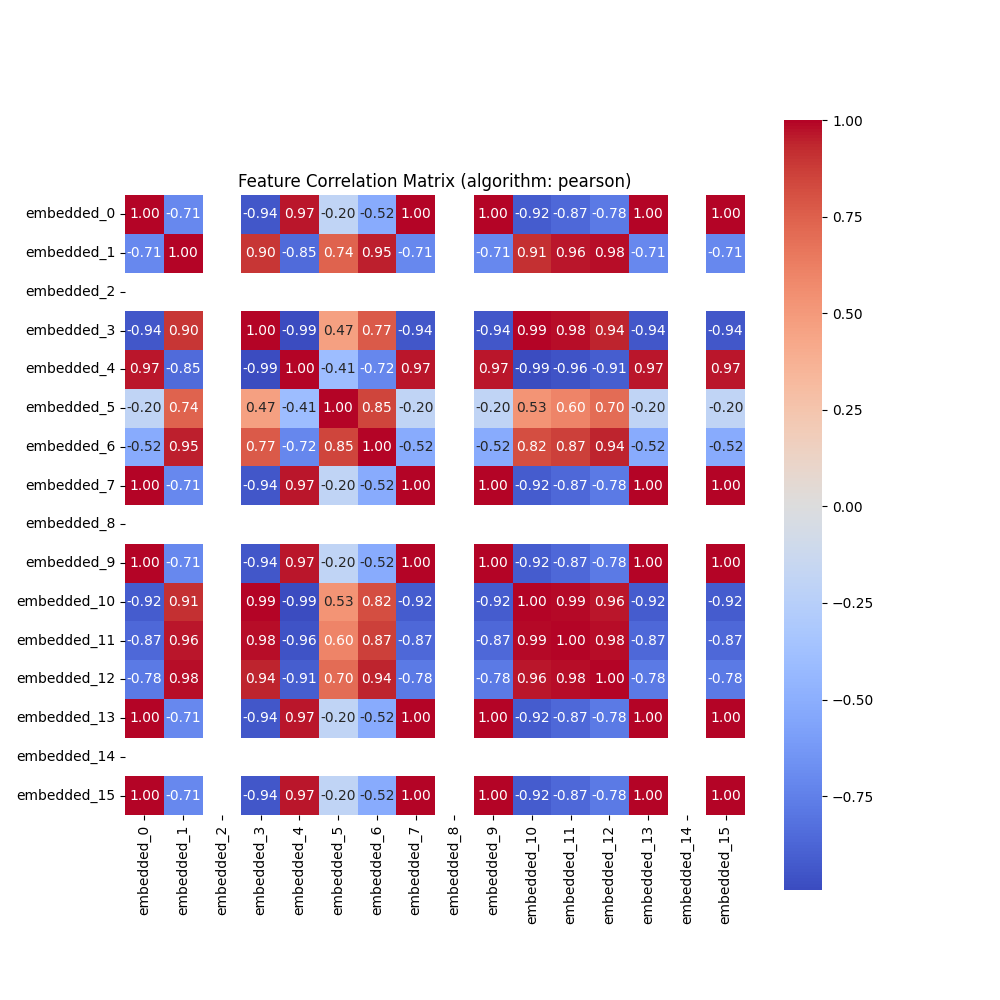
\includegraphics[width=0.8\linewidth]{img/annexes/26/Transformers 1_correlation_matrix.png}} \\
\hline
\end{longtable}


\begin{longtable}{|c|c|}
\caption{Word2vec 1 Feature Engineering Results on 26} \label{tab:26_word2vec_1_feature_engineering_results}\\
\hline
Dataset Name & 26 \\ \hline
Instance & Word2vec 1 \\ \hline
\multirow{8}{*}{Best Features} & feature\_4 \\ \cline{2-2}
 & feature\_5 \\ \cline{2-2}
 & feature\_6 \\ \cline{2-2}
 & feature\_7 \\ \cline{2-2}
 & feature\_2 \\ \cline{2-2}
 & feature\_3 \\ \cline{2-2}
 & feature\_0 \\ \cline{2-2}
 & feature\_1 \\ \cline{2-2}
\noalign{\vskip 5mm}
\multicolumn{2}{|c|}{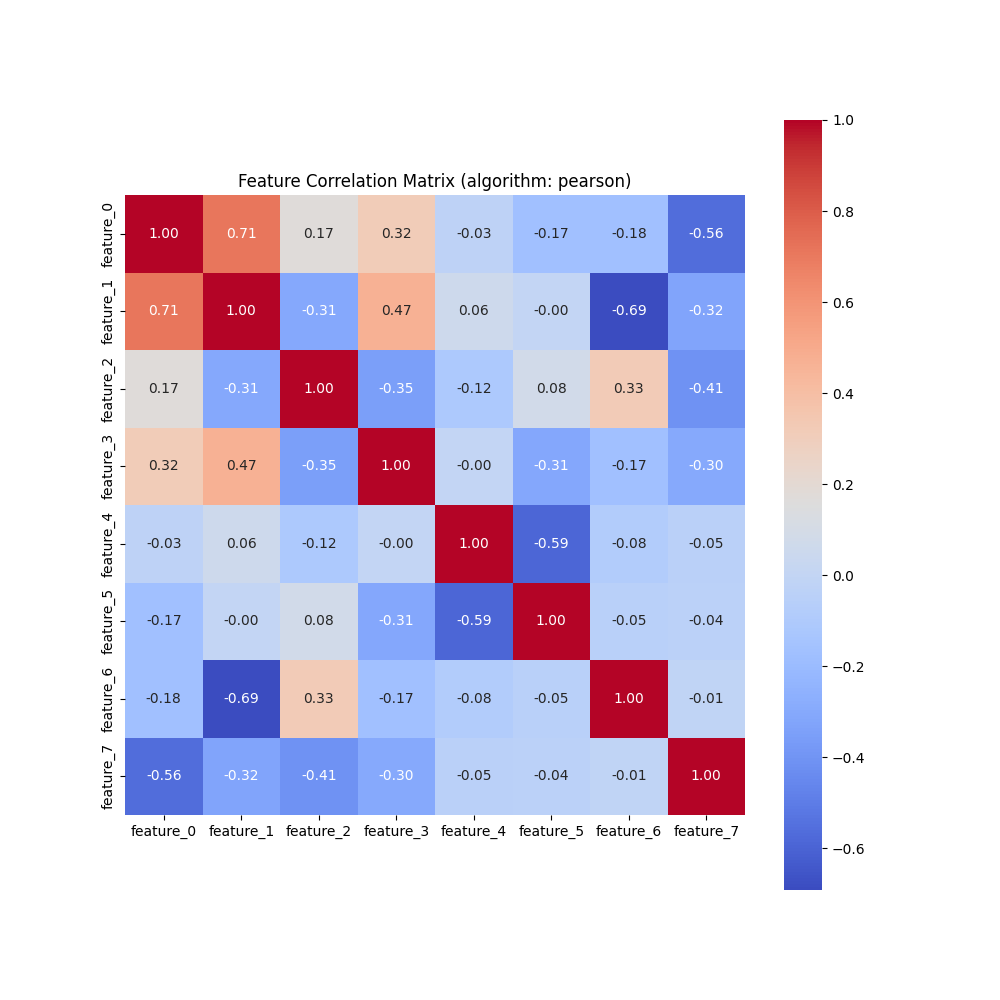
\includegraphics[width=0.8\linewidth]{img/annexes/26/Word2vec 1_correlation_matrix.png}} \\
\hline
\end{longtable}


\subsection{24 chunk\_extraction}

\subsection{25 chunk\_extraction (filtered chunk size)}

\begin{longtable}{|c|c|}
\caption{Word2vec 3 Feature Engineering Results on 25} \label{tab:25_word2vec_3_feature_engineering_results}\\
\hline
Dataset Name & 25 \\ \hline
Instance & Word2vec 3 \\ \hline
\multirow{8}{*}{Best Features} & feature\_2 \\ \cline{2-2}
 & feature\_5 \\ \cline{2-2}
 & feature\_3 \\ \cline{2-2}
 & feature\_6 \\ \cline{2-2}
 & feature\_7 \\ \cline{2-2}
 & feature\_4 \\ \cline{2-2}
 & feature\_0 \\ \cline{2-2}
 & feature\_1 \\ \cline{2-2}
\noalign{\vskip 5mm}
\multicolumn{2}{|c|}{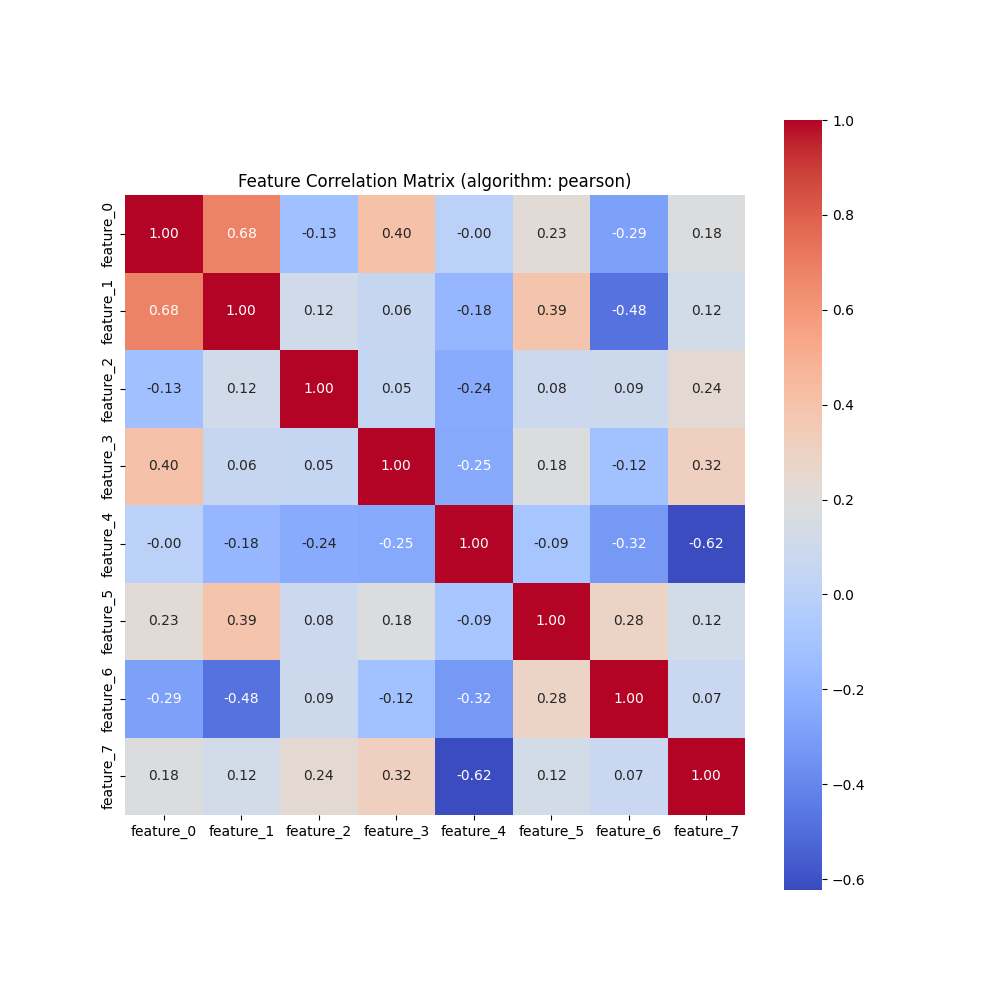
\includegraphics[width=0.8\linewidth]{img/annexes/25/Word2vec 3_correlation_matrix.png}} \\
\hline
\end{longtable}


\subsection{27 chunk\_extraction (filtered entropy and chunk size)}

\begin{longtable}{|c|c|}
\caption{Transformers 1 Feature Engineering Results on 27} \label{tab:27_transformers_1_feature_engineering_results}\\
\hline
Dataset Name & 27 \\ \hline
Instance & Transformers 1 \\ \hline
\multirow{8}{*}{Best Features} & embedded\_0 \\ \cline{2-2}
 & embedded\_6 \\ \cline{2-2}
 & embedded\_7 \\ \cline{2-2}
 & embedded\_9 \\ \cline{2-2}
 & embedded\_8 \\ \cline{2-2}
 & embedded\_10 \\ \cline{2-2}
 & embedded\_5 \\ \cline{2-2}
 & embedded\_3 \\ \cline{2-2}
\noalign{\vskip 5mm}
\multicolumn{2}{|c|}{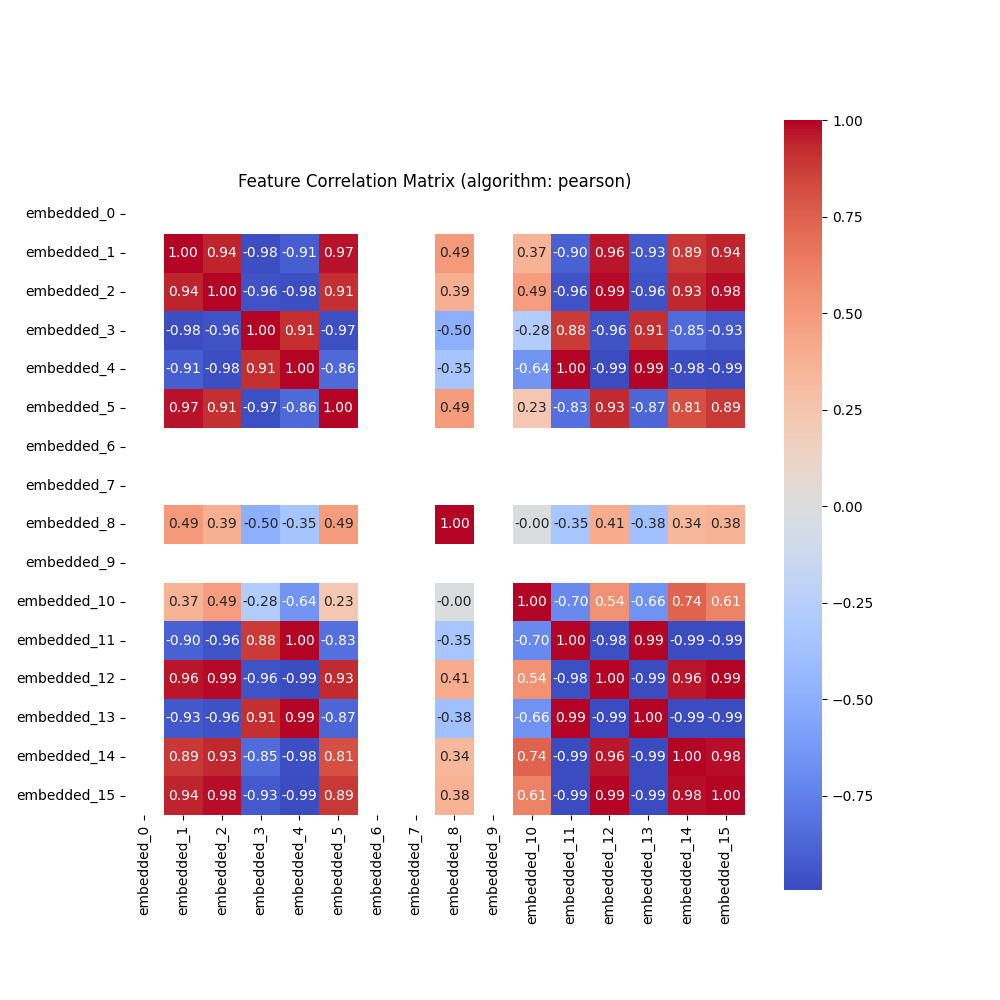
\includegraphics[width=0.8\linewidth]{img/annexes/27/Transformers 1_correlation_matrix.png}} \\
\hline
\end{longtable}


\begin{longtable}{|c|c|}
\caption{Word2vec 3 Feature Engineering Results on 27} \label{tab:27_word2vec_3_feature_engineering_results}\\
\hline
Dataset Name & 27 \\ \hline
Instance & Word2vec 3 \\ \hline
\multirow{8}{*}{Best Features} & feature\_4 \\ \cline{2-2}
 & feature\_3 \\ \cline{2-2}
 & feature\_1 \\ \cline{2-2}
 & feature\_2 \\ \cline{2-2}
 & feature\_0 \\ \cline{2-2}
 & feature\_6 \\ \cline{2-2}
 & feature\_7 \\ \cline{2-2}
 & feature\_5 \\ \cline{2-2}
\noalign{\vskip 5mm}
\multicolumn{2}{|c|}{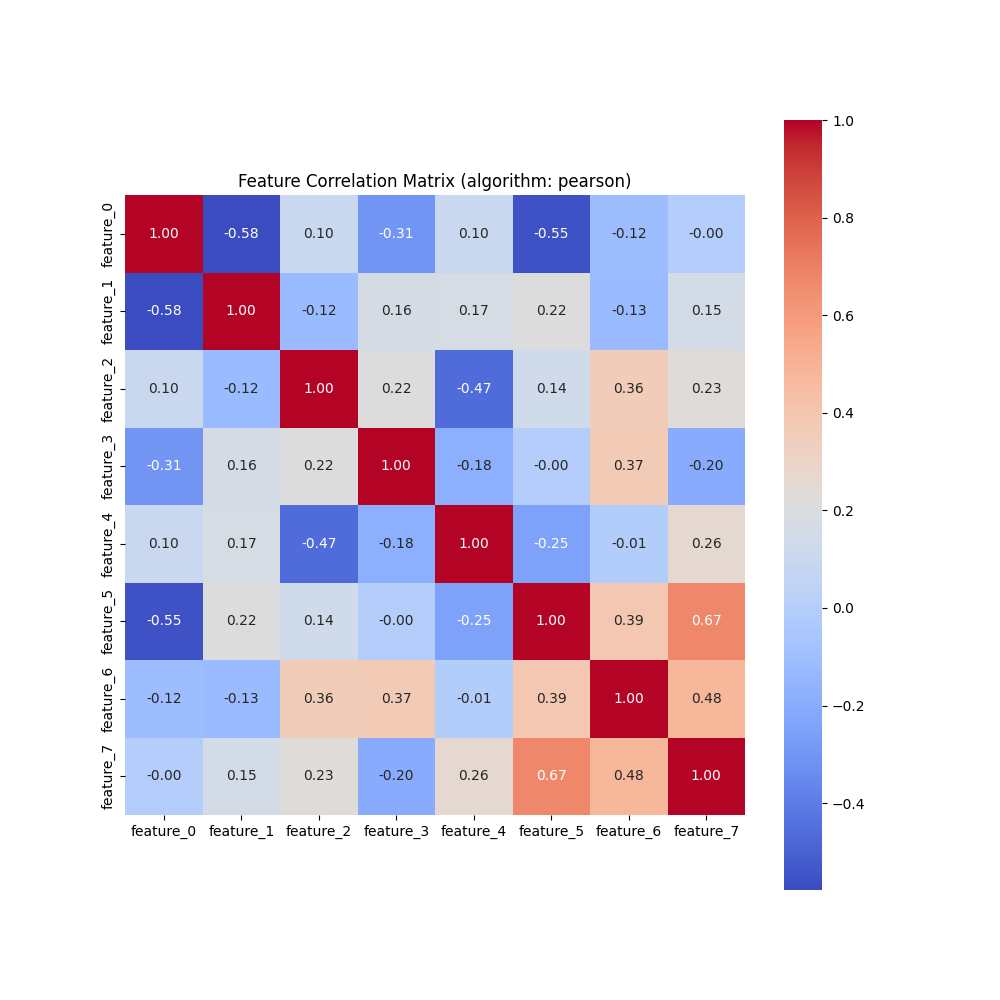
\includegraphics[width=0.8\linewidth]{img/annexes/27/Word2vec 3_correlation_matrix.png}} \\
\hline
\end{longtable}


\section{Clustering results}

\label{sec:annexe:clustering_results}

\subsection{26 chunk\_extraction (filtered entropy)}

\begin{longtable}{|c|c|c|c|c|}
\caption{Transformers 0 Clustering Results on 26} \label{tab:26_transformers_0_clustering_results}\\
\hline
\multicolumn{5}{|c|}{\textbf{General Information}} \\
\hline
\multicolumn{2}{|c|}{Min Samples} & \multicolumn{3}{c|}{937} \\
\multicolumn{2}{|c|}{Total Duration} & \multicolumn{3}{c|}{3588.869441 s} \\
\hline
\multicolumn{5}{|c|}{\textbf{Clustering Information}} \\
\hline
EPS & Number of Clusters & Silhouette Score & Noise Points & Duration \\
0.01 & 3 & 0.5749053359031677 & 1369 & 674.16573 s\\
0.02 & 3 & 0.5749053359031677 & 1369 & 664.292675 s\\
0.03 & 3 & 0.574790894985199 & 1371 & 699.778419 s\\
0.04 & 3 & 0.574790894985199 & 1371 & 770.27842 s\\
0.05 & 3 & 0.574790894985199 & 1371 & 776.637103 s\\
\hline
\multicolumn{5}{|c|}{\textbf{Best EPS Information}} \\
\hline
0.01 & 3 & 0.5749053359031677 & 1369 & 674.16573 s\\
\hline
\multicolumn{5}{|c|}{\textbf{Label Association}} \\
\hline
Cluster ID & \multicolumn{2}{c|}{Label} & \multicolumn{2}{c|}{Number of Samples} \\
\hline
\multirow{4}{*}{-1.0} & \multicolumn{2}{c|}{0.0} & \multicolumn{2}{c|}{31} \\
& \multicolumn{2}{c|}{1.0} & \multicolumn{2}{c|}{40} \\
& \multicolumn{2}{c|}{2.0} & \multicolumn{2}{c|}{56} \\
& \multicolumn{2}{c|}{4.0} & \multicolumn{2}{c|}{33} \\
\hline
\multirow{4}{*}{0.0} & \multicolumn{2}{c|}{0.0} & \multicolumn{2}{c|}{35} \\
& \multicolumn{2}{c|}{1.0} & \multicolumn{2}{c|}{40} \\
& \multicolumn{2}{c|}{2.0} & \multicolumn{2}{c|}{26} \\
& \multicolumn{2}{c|}{4.0} & \multicolumn{2}{c|}{32} \\
\hline
\multirow{4}{*}{1.0} & \multicolumn{2}{c|}{0.0} & \multicolumn{2}{c|}{77} \\
& \multicolumn{2}{c|}{1.0} & \multicolumn{2}{c|}{91} \\
& \multicolumn{2}{c|}{2.0} & \multicolumn{2}{c|}{76} \\
& \multicolumn{2}{c|}{4.0} & \multicolumn{2}{c|}{96} \\
\hline
\multirow{4}{*}{2.0} & \multicolumn{2}{c|}{0.0} & \multicolumn{2}{c|}{32} \\
& \multicolumn{2}{c|}{1.0} & \multicolumn{2}{c|}{45} \\
& \multicolumn{2}{c|}{2.0} & \multicolumn{2}{c|}{45} \\
& \multicolumn{2}{c|}{4.0} & \multicolumn{2}{c|}{42} \\
\hline
\multicolumn{5}{|c|}{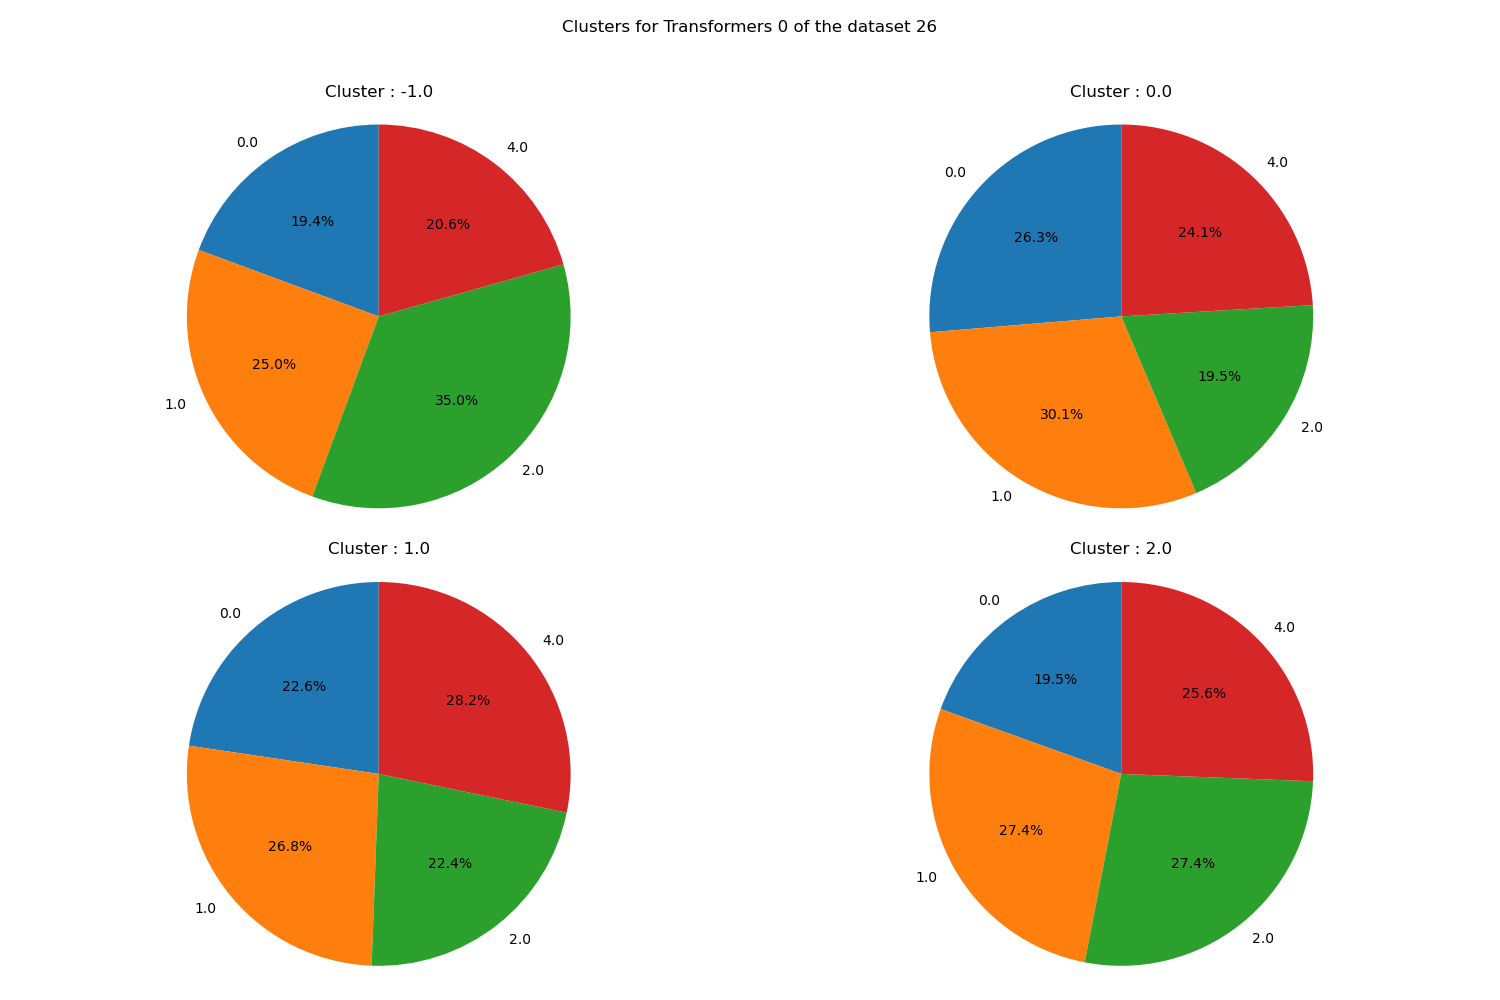
\includegraphics[width=0.8\linewidth]{img/annexes/26/clustering_pie_charts/Transformers 0.png}} \\
\end{longtable}


\begin{longtable}{|c|c|c|c|c|}
\caption{Transformers 1 Clustering Results on 26} \label{tab:26_transformers_1_clustering_results}\\
\hline
\multicolumn{5}{|c|}{\textbf{General Information}} \\
\hline
\multicolumn{2}{|c|}{Min Samples} & \multicolumn{3}{c|}{937} \\
\multicolumn{2}{|c|}{Total Duration} & \multicolumn{3}{c|}{3739.406415 s} \\
\hline
\multicolumn{5}{|c|}{\textbf{Clustering Information}} \\
\hline
EPS & Number of Clusters & Silhouette Score & Noise Points & Duration \\
0.01 & 3 & 0.7379494309425354 & 1299 & 760.134469 s\\
0.02 & 3 & 0.7379494309425354 & 1299 & 731.259721 s\\
0.03 & 3 & 0.7379494309425354 & 1299 & 738.923279 s\\
0.04 & 3 & 0.7379494309425354 & 1299 & 761.430407 s\\
0.05 & 3 & 0.3740614056587219 & 2696 & 743.313265 s\\
\hline
\multicolumn{5}{|c|}{\textbf{Best EPS Information}} \\
\hline
0.01 & 3 & 0.7379494309425354 & 1299 & 760.134469 s\\
\hline
\multicolumn{5}{|c|}{\textbf{Label Association}} \\
\hline
Cluster ID & \multicolumn{2}{c|}{Label} & \multicolumn{2}{c|}{Number of Samples} \\
\hline
\multirow{4}{*}{-1.0} & \multicolumn{2}{c|}{0.0} & \multicolumn{2}{c|}{29} \\
& \multicolumn{2}{c|}{1.0} & \multicolumn{2}{c|}{37} \\
& \multicolumn{2}{c|}{2.0} & \multicolumn{2}{c|}{56} \\
& \multicolumn{2}{c|}{4.0} & \multicolumn{2}{c|}{32} \\
\hline
\multirow{4}{*}{0.0} & \multicolumn{2}{c|}{0.0} & \multicolumn{2}{c|}{37} \\
& \multicolumn{2}{c|}{1.0} & \multicolumn{2}{c|}{43} \\
& \multicolumn{2}{c|}{2.0} & \multicolumn{2}{c|}{26} \\
& \multicolumn{2}{c|}{4.0} & \multicolumn{2}{c|}{33} \\
\hline
\multirow{4}{*}{1.0} & \multicolumn{2}{c|}{0.0} & \multicolumn{2}{c|}{77} \\
& \multicolumn{2}{c|}{1.0} & \multicolumn{2}{c|}{91} \\
& \multicolumn{2}{c|}{2.0} & \multicolumn{2}{c|}{76} \\
& \multicolumn{2}{c|}{4.0} & \multicolumn{2}{c|}{96} \\
\hline
\multirow{4}{*}{2.0} & \multicolumn{2}{c|}{0.0} & \multicolumn{2}{c|}{32} \\
& \multicolumn{2}{c|}{1.0} & \multicolumn{2}{c|}{45} \\
& \multicolumn{2}{c|}{2.0} & \multicolumn{2}{c|}{45} \\
& \multicolumn{2}{c|}{4.0} & \multicolumn{2}{c|}{42} \\
\hline
\multicolumn{5}{|c|}{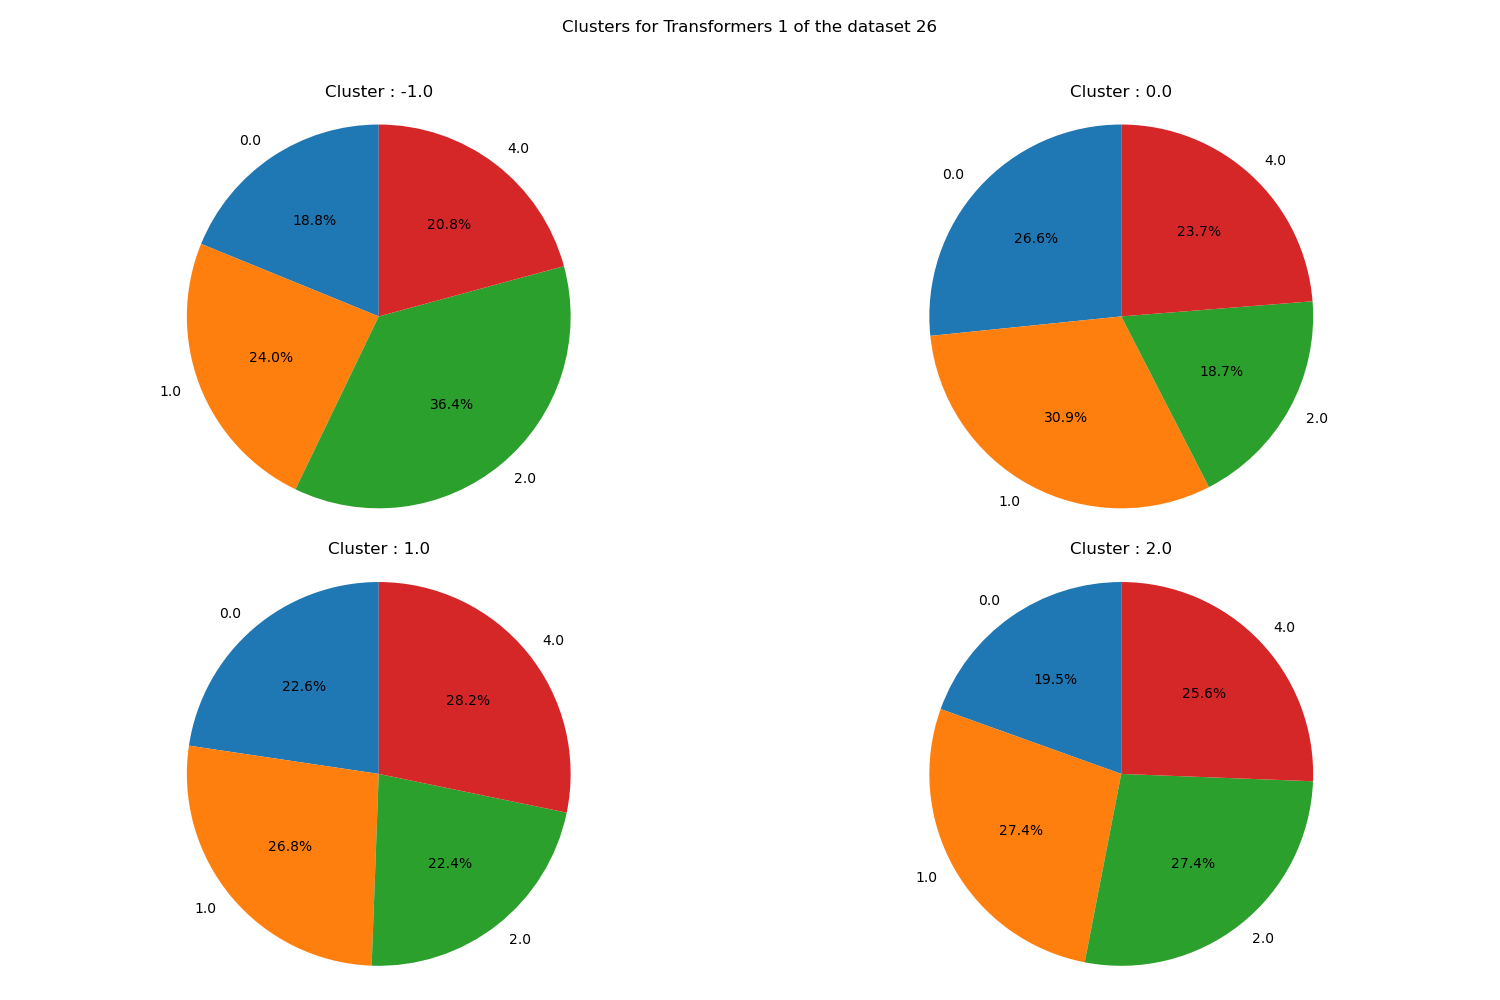
\includegraphics[width=0.8\linewidth]{img/annexes/26/clustering_pie_charts/Transformers 1.png}} \\
\end{longtable}


\subsection{24 chunk\_extraction}

\subsection{25 chunk\_extraction (filtered chunk size)}

\begin{longtable}{|c|c|c|c|c|}
\caption{Word2vec 3 Clustering Results on 25} \label{tab:25_word2vec_3_clustering_results}\\
\hline
\multicolumn{5}{|c|}{\textbf{General Information}} \\
\hline
\multicolumn{2}{|c|}{Min Samples} & \multicolumn{3}{c|}{937} \\
\multicolumn{2}{|c|}{Total Duration} & \multicolumn{3}{c|}{3634.492193 s} \\
\hline
\multicolumn{5}{|c|}{\textbf{Clustering Information}} \\
\hline
EPS & Number of Clusters & Silhouette Score & Noise Points & Duration \\
0.01 & 2 & 0.21665062010288239 & 3676 & 747.692523 s\\
0.02 & 1 & None & None & 697.073419 s\\
0.03 & 1 & None & None & 694.980969 s\\
0.04 & 1 & None & None & 737.728848 s\\
0.05 & 1 & None & None & 756.257249 s\\
\hline
\multicolumn{5}{|c|}{\textbf{Best EPS Information}} \\
\hline
0.01 & 2 & 0.21665062010288239 & 3676 & 747.692523 s\\
\hline
\multicolumn{5}{|c|}{\textbf{Label Association}} \\
\hline
Cluster ID & \multicolumn{2}{c|}{Label} & \multicolumn{2}{c|}{Number of Samples} \\
\hline
\multirow{4}{*}{-1.0} & \multicolumn{2}{c|}{0.0} & \multicolumn{2}{c|}{3} \\
& \multicolumn{2}{c|}{1.0} & \multicolumn{2}{c|}{2} \\
& \multicolumn{2}{c|}{2.0} & \multicolumn{2}{c|}{1} \\
& \multicolumn{2}{c|}{4.0} & \multicolumn{2}{c|}{2} \\
\hline
\multirow{2}{*}{0.0} & \multicolumn{2}{c|}{2.0} & \multicolumn{2}{c|}{2} \\
& \multicolumn{2}{c|}{4.0} & \multicolumn{2}{c|}{1} \\
\hline
\multirow{1}{*}{1.0} & \multicolumn{2}{c|}{0.0} & \multicolumn{2}{c|}{2} \\
\hline
\multicolumn{5}{|c|}{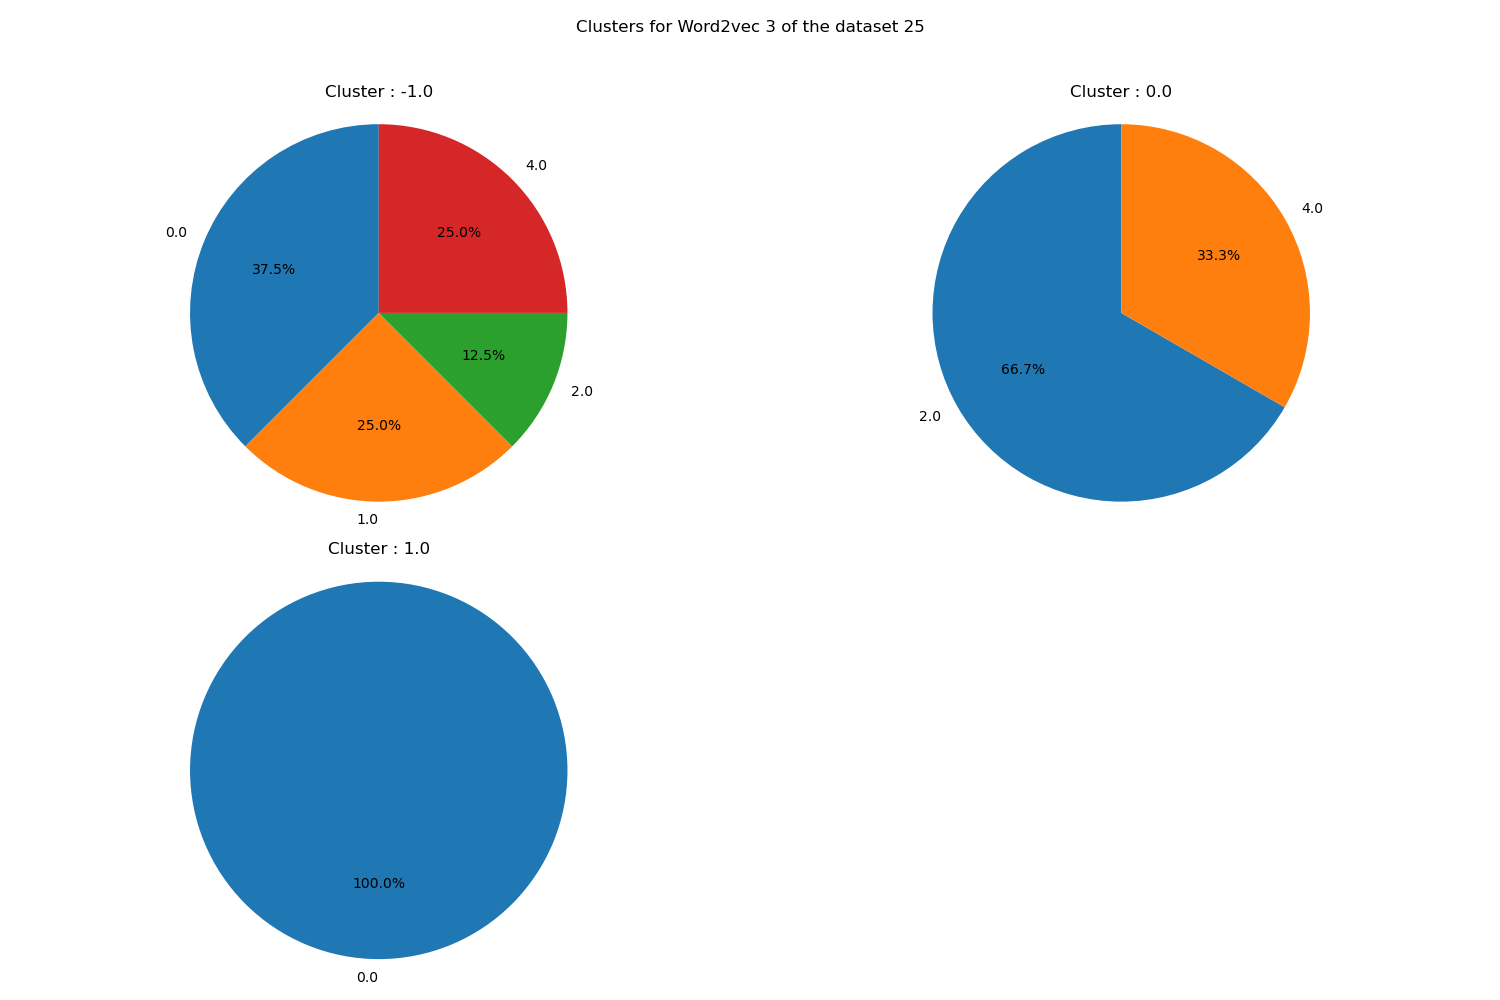
\includegraphics[width=0.8\linewidth]{img/annexes/25/clustering_pie_charts/Word2vec 3.png}} \\
\end{longtable}


\subsection{27 chunk\_extraction (filtered entropy and chunk size)}

\begin{longtable}{|c|c|c|c|c|}
\caption{Transformers 0 Clustering Results on 27} \label{tab:27_transformers_0_clustering_results}\\
\hline
\multicolumn{5}{|c|}{\textbf{General Information}} \\
\hline
\multicolumn{2}{|c|}{Min Samples} & \multicolumn{3}{c|}{937} \\
\multicolumn{2}{|c|}{Total Duration} & \multicolumn{3}{c|}{3796.324605 s} \\
\hline
\multicolumn{5}{|c|}{\textbf{Clustering Information}} \\
\hline
EPS & Number of Clusters & Silhouette Score & Noise Points & Duration \\
0.01 & 3 & 0.2465989887714386 & 2274 & 709.617939 s\\
0.02 & 3 & 0.24514129757881165 & 2281 & 753.217155 s\\
0.03 & 2 & 0.1906411200761795 & 3242 & 820.552446 s\\
0.04 & 2 & 0.1906411200761795 & 3242 & 756.897654 s\\
0.05 & 2 & 0.1906411200761795 & 3242 & 751.836631 s\\
\hline
\multicolumn{5}{|c|}{\textbf{Best EPS Information}} \\
\hline
0.01 & 3 & 0.2465989887714386 & 2274 & 709.617939 s\\
\hline
\multicolumn{5}{|c|}{\textbf{Label Association}} \\
\hline
Cluster ID & \multicolumn{2}{c|}{Label} & \multicolumn{2}{c|}{Number of Samples} \\
\hline
\multirow{4}{*}{-1.0} & \multicolumn{2}{c|}{0.0} & \multicolumn{2}{c|}{91} \\
& \multicolumn{2}{c|}{1.0} & \multicolumn{2}{c|}{95} \\
& \multicolumn{2}{c|}{2.0} & \multicolumn{2}{c|}{99} \\
& \multicolumn{2}{c|}{4.0} & \multicolumn{2}{c|}{97} \\
\hline
\multirow{4}{*}{0.0} & \multicolumn{2}{c|}{0.0} & \multicolumn{2}{c|}{128} \\
& \multicolumn{2}{c|}{1.0} & \multicolumn{2}{c|}{129} \\
& \multicolumn{2}{c|}{2.0} & \multicolumn{2}{c|}{94} \\
& \multicolumn{2}{c|}{4.0} & \multicolumn{2}{c|}{110} \\
\hline
\multirow{4}{*}{1.0} & \multicolumn{2}{c|}{0.0} & \multicolumn{2}{c|}{50} \\
& \multicolumn{2}{c|}{1.0} & \multicolumn{2}{c|}{40} \\
& \multicolumn{2}{c|}{2.0} & \multicolumn{2}{c|}{44} \\
& \multicolumn{2}{c|}{4.0} & \multicolumn{2}{c|}{33} \\
\hline
\multirow{4}{*}{2.0} & \multicolumn{2}{c|}{0.0} & \multicolumn{2}{c|}{52} \\
& \multicolumn{2}{c|}{1.0} & \multicolumn{2}{c|}{51} \\
& \multicolumn{2}{c|}{2.0} & \multicolumn{2}{c|}{53} \\
& \multicolumn{2}{c|}{4.0} & \multicolumn{2}{c|}{50} \\
\hline
\multicolumn{5}{|c|}{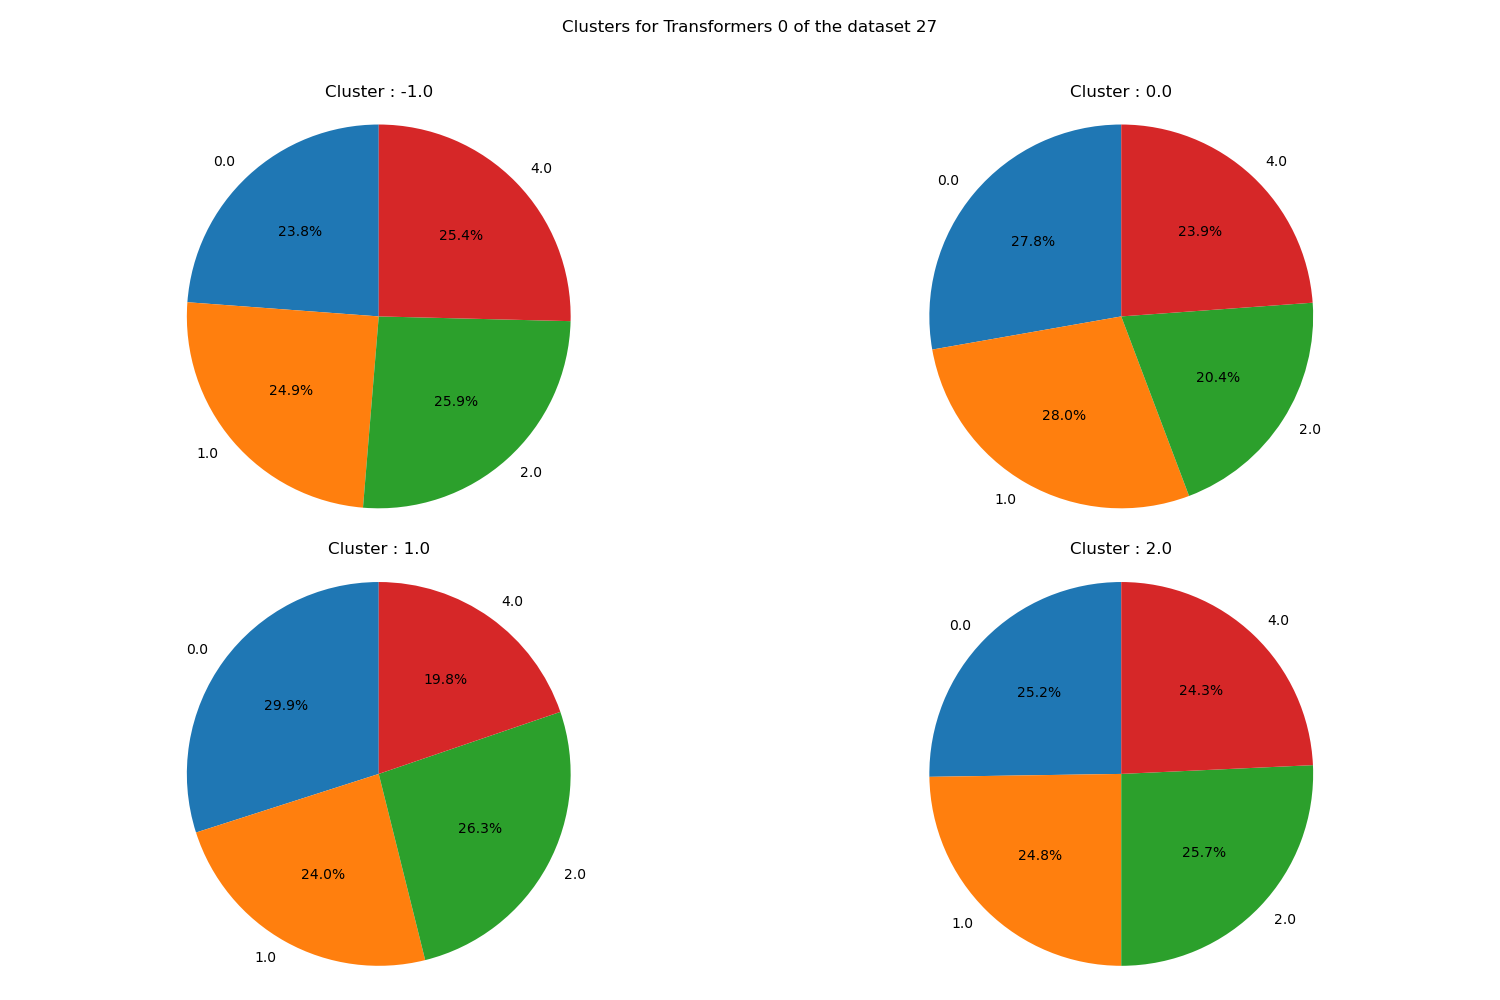
\includegraphics[width=0.8\linewidth]{img/annexes/27/clustering_pie_charts/Transformers 0.png}} \\
\end{longtable}


\begin{longtable}{|c|c|c|c|c|}
\caption{Transformers 1 Clustering Results on 27} \label{tab:27_transformers_1_clustering_results}\\
\hline
\multicolumn{5}{|c|}{\textbf{General Information}} \\
\hline
\multicolumn{2}{|c|}{Min Samples} & \multicolumn{3}{c|}{937} \\
\multicolumn{2}{|c|}{Total Duration} & \multicolumn{3}{c|}{3943.383724 s} \\
\hline
\multicolumn{5}{|c|}{\textbf{Clustering Information}} \\
\hline
EPS & Number of Clusters & Silhouette Score & Noise Points & Duration \\
0.01 & 4 & 0.5144023299217224 & 981 & 810.887225 s\\
0.02 & 3 & 0.8070926070213318 & 533 & 798.792131 s\\
0.03 & 3 & 0.8070926070213318 & 533 & 772.422919 s\\
0.04 & 3 & 0.8070926070213318 & 533 & 775.663572 s\\
0.05 & 3 & 0.8070926070213318 & 533 & 781.48437 s\\
\hline
\multicolumn{5}{|c|}{\textbf{Best EPS Information}} \\
\hline
0.02 & 3 & 0.8070926070213318 & 533 & 798.792131 s\\
\hline
\multicolumn{5}{|c|}{\textbf{Label Association}} \\
\hline
Cluster ID & \multicolumn{2}{c|}{Label} & \multicolumn{2}{c|}{Number of Samples} \\
\hline
\multirow{4}{*}{-1.0} & \multicolumn{2}{c|}{0.0} & \multicolumn{2}{c|}{19} \\
& \multicolumn{2}{c|}{1.0} & \multicolumn{2}{c|}{20} \\
& \multicolumn{2}{c|}{2.0} & \multicolumn{2}{c|}{20} \\
& \multicolumn{2}{c|}{4.0} & \multicolumn{2}{c|}{20} \\
\hline
\multirow{4}{*}{0.0} & \multicolumn{2}{c|}{0.0} & \multicolumn{2}{c|}{182} \\
& \multicolumn{2}{c|}{1.0} & \multicolumn{2}{c|}{155} \\
& \multicolumn{2}{c|}{2.0} & \multicolumn{2}{c|}{138} \\
& \multicolumn{2}{c|}{4.0} & \multicolumn{2}{c|}{145} \\
\hline
\multirow{4}{*}{1.0} & \multicolumn{2}{c|}{0.0} & \multicolumn{2}{c|}{74} \\
& \multicolumn{2}{c|}{1.0} & \multicolumn{2}{c|}{96} \\
& \multicolumn{2}{c|}{2.0} & \multicolumn{2}{c|}{81} \\
& \multicolumn{2}{c|}{4.0} & \multicolumn{2}{c|}{85} \\
\hline
\multirow{4}{*}{2.0} & \multicolumn{2}{c|}{0.0} & \multicolumn{2}{c|}{46} \\
& \multicolumn{2}{c|}{1.0} & \multicolumn{2}{c|}{44} \\
& \multicolumn{2}{c|}{2.0} & \multicolumn{2}{c|}{51} \\
& \multicolumn{2}{c|}{4.0} & \multicolumn{2}{c|}{40} \\
\hline
\multicolumn{5}{|c|}{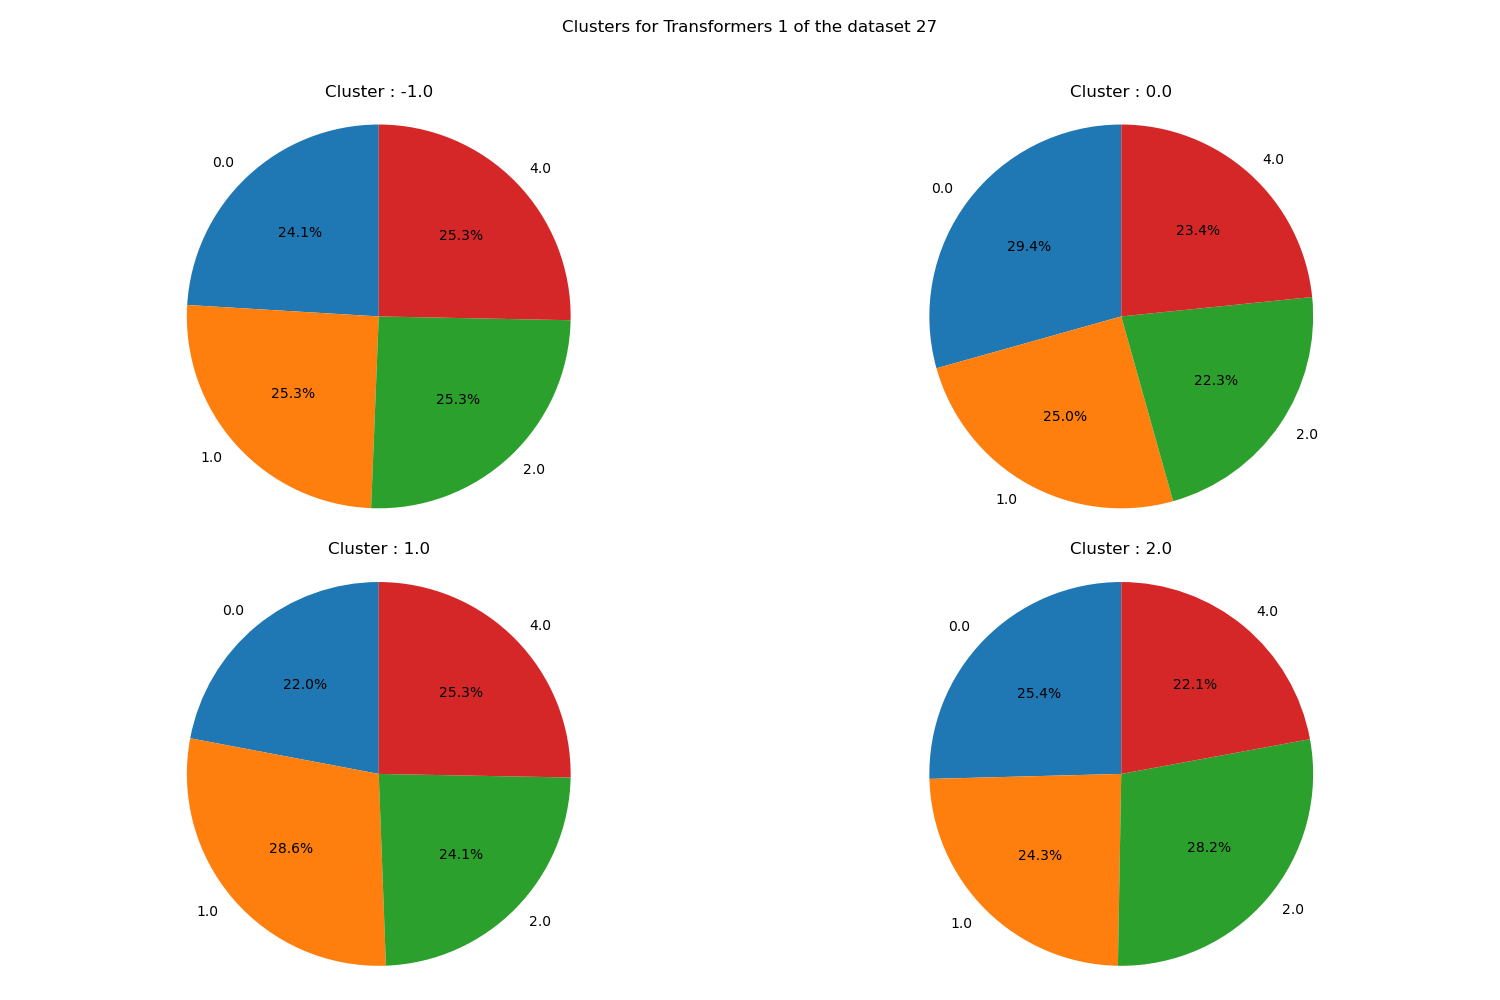
\includegraphics[width=0.8\linewidth]{img/annexes/27/clustering_pie_charts/Transformers 1.png}} \\
\end{longtable}


\begin{longtable}{|c|c|c|c|c|}
\caption{Transformers 2 Clustering Results on 27} \label{tab:27_transformers_2_clustering_results}\\
\hline
\multicolumn{5}{|c|}{\textbf{General Information}} \\
\hline
\multicolumn{2}{|c|}{Min Samples} & \multicolumn{3}{c|}{937} \\
\multicolumn{2}{|c|}{Total Duration} & \multicolumn{3}{c|}{3895.618311 s} \\
\hline
\multicolumn{5}{|c|}{\textbf{Clustering Information}} \\
\hline
EPS & Number of Clusters & Silhouette Score & Noise Points & Duration \\
0.01 & 2 & 0.907838761806488 & 0 & 790.283896 s\\
0.02 & 2 & 0.907838761806488 & 0 & 802.295121 s\\
0.03 & 2 & 0.907838761806488 & 0 & 787.142639 s\\
0.04 & 2 & 0.907838761806488 & 0 & 725.182204 s\\
0.05 & 2 & 0.907838761806488 & 0 & 785.995246 s\\
\hline
\multicolumn{5}{|c|}{\textbf{Best EPS Information}} \\
\hline
0.01 & 2 & 0.907838761806488 & 0 & 790.283896 s\\
\hline
\multicolumn{5}{|c|}{\textbf{Label Association}} \\
\hline
Cluster ID & \multicolumn{2}{c|}{Label} & \multicolumn{2}{c|}{Number of Samples} \\
\hline
\multirow{4}{*}{0.0} & \multicolumn{2}{c|}{0.0} & \multicolumn{2}{c|}{264} \\
& \multicolumn{2}{c|}{1.0} & \multicolumn{2}{c|}{256} \\
& \multicolumn{2}{c|}{2.0} & \multicolumn{2}{c|}{228} \\
& \multicolumn{2}{c|}{4.0} & \multicolumn{2}{c|}{236} \\
\hline
\multirow{4}{*}{1.0} & \multicolumn{2}{c|}{0.0} & \multicolumn{2}{c|}{57} \\
& \multicolumn{2}{c|}{1.0} & \multicolumn{2}{c|}{59} \\
& \multicolumn{2}{c|}{2.0} & \multicolumn{2}{c|}{62} \\
& \multicolumn{2}{c|}{4.0} & \multicolumn{2}{c|}{54} \\
\hline
\multicolumn{5}{|c|}{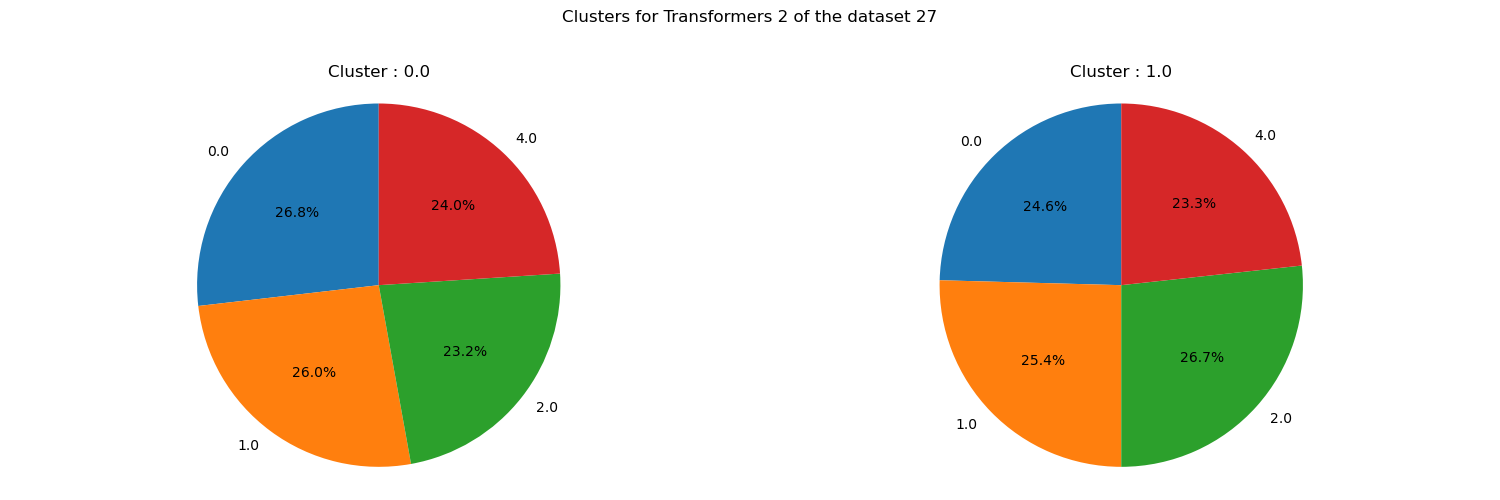
\includegraphics[width=0.8\linewidth]{img/annexes/27/clustering_pie_charts/Transformers 2.png}} \\
\end{longtable}


\begin{longtable}{|c|c|c|c|c|}
\caption{Transformers 3 Clustering Results on 27} \label{tab:27_transformers_3_clustering_results}\\
\hline
\multicolumn{5}{|c|}{\textbf{General Information}} \\
\hline
\multicolumn{2}{|c|}{Min Samples} & \multicolumn{3}{c|}{937} \\
\multicolumn{2}{|c|}{Total Duration} & \multicolumn{3}{c|}{3939.333846 s} \\
\hline
\multicolumn{5}{|c|}{\textbf{Clustering Information}} \\
\hline
EPS & Number of Clusters & Silhouette Score & Noise Points & Duration \\
0.01 & 3 & 0.36908280849456787 & 2637 & 806.707338 s\\
0.02 & 3 & 0.36908280849456787 & 2637 & 782.581847 s\\
0.03 & 3 & 0.36908280849456787 & 2637 & 775.659231 s\\
0.04 & 3 & 0.36908280849456787 & 2637 & 783.727976 s\\
0.05 & 3 & 0.36908280849456787 & 2637 & 786.255646 s\\
\hline
\multicolumn{5}{|c|}{\textbf{Best EPS Information}} \\
\hline
0.01 & 3 & 0.36908280849456787 & 2637 & 806.707338 s\\
\hline
\multicolumn{5}{|c|}{\textbf{Label Association}} \\
\hline
Cluster ID & \multicolumn{2}{c|}{Label} & \multicolumn{2}{c|}{Number of Samples} \\
\hline
\multirow{4}{*}{-1.0} & \multicolumn{2}{c|}{0.0} & \multicolumn{2}{c|}{134} \\
& \multicolumn{2}{c|}{1.0} & \multicolumn{2}{c|}{97} \\
& \multicolumn{2}{c|}{2.0} & \multicolumn{2}{c|}{114} \\
& \multicolumn{2}{c|}{4.0} & \multicolumn{2}{c|}{111} \\
\hline
\multirow{4}{*}{0.0} & \multicolumn{2}{c|}{0.0} & \multicolumn{2}{c|}{81} \\
& \multicolumn{2}{c|}{1.0} & \multicolumn{2}{c|}{86} \\
& \multicolumn{2}{c|}{2.0} & \multicolumn{2}{c|}{53} \\
& \multicolumn{2}{c|}{4.0} & \multicolumn{2}{c|}{72} \\
\hline
\multirow{4}{*}{1.0} & \multicolumn{2}{c|}{0.0} & \multicolumn{2}{c|}{49} \\
& \multicolumn{2}{c|}{1.0} & \multicolumn{2}{c|}{73} \\
& \multicolumn{2}{c|}{2.0} & \multicolumn{2}{c|}{61} \\
& \multicolumn{2}{c|}{4.0} & \multicolumn{2}{c|}{53} \\
\hline
\multirow{4}{*}{2.0} & \multicolumn{2}{c|}{0.0} & \multicolumn{2}{c|}{57} \\
& \multicolumn{2}{c|}{1.0} & \multicolumn{2}{c|}{59} \\
& \multicolumn{2}{c|}{2.0} & \multicolumn{2}{c|}{62} \\
& \multicolumn{2}{c|}{4.0} & \multicolumn{2}{c|}{54} \\
\hline
\multicolumn{5}{|c|}{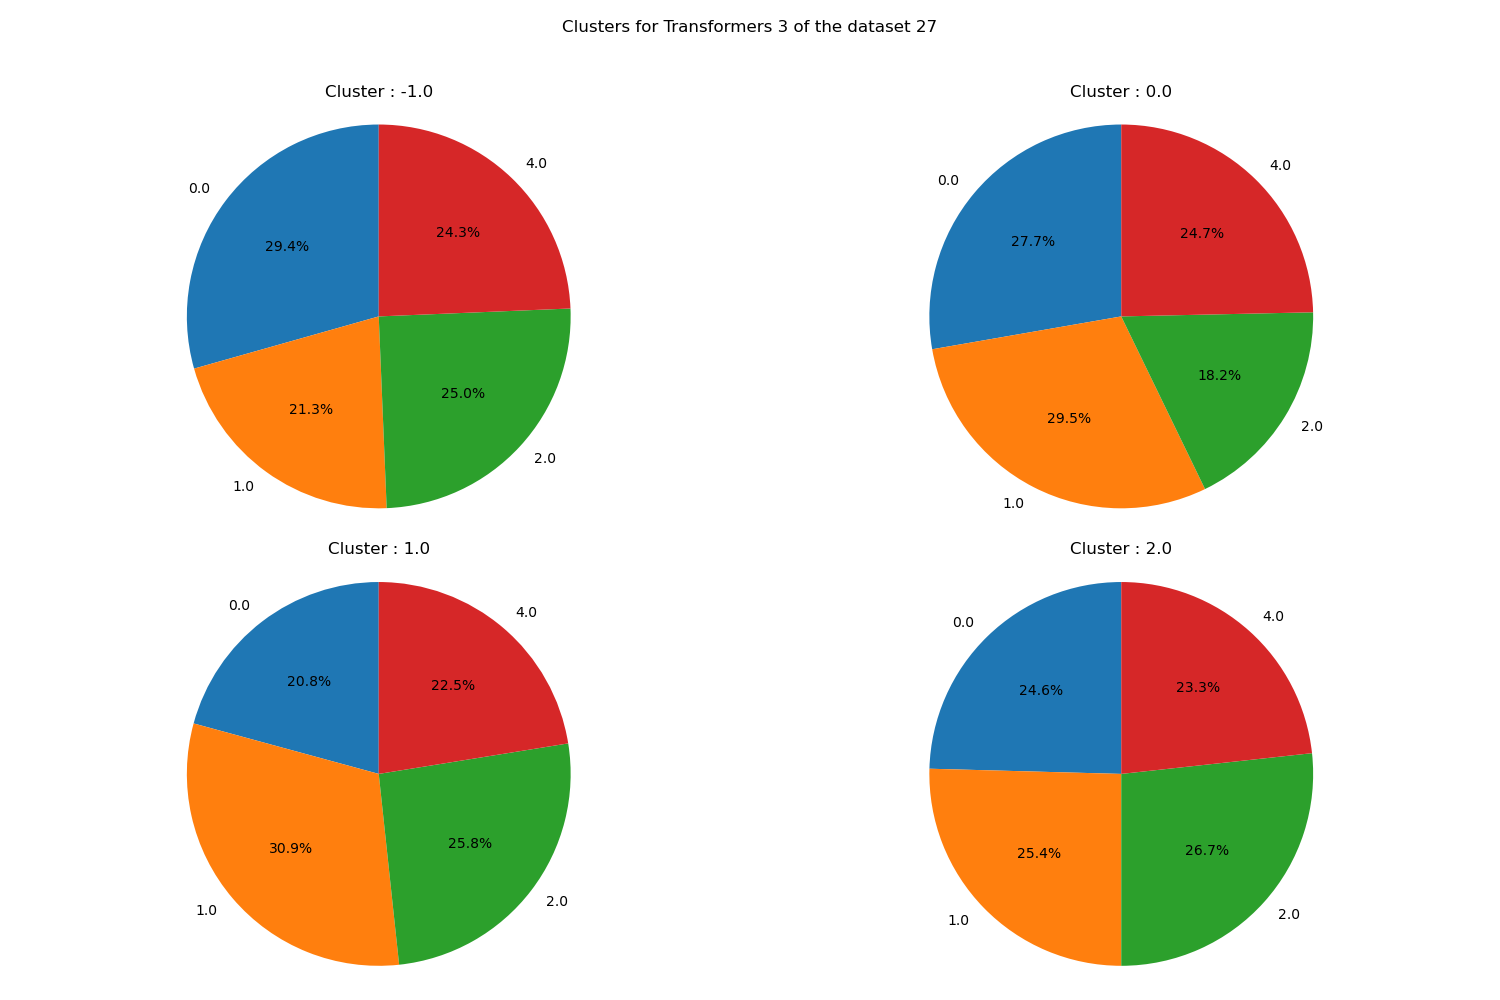
\includegraphics[width=0.8\linewidth]{img/annexes/27/clustering_pie_charts/Transformers 3.png}} \\
\end{longtable}


\begin{longtable}{|c|c|c|c|c|}
\caption{Transformers 4 Clustering Results on 27} \label{tab:27_transformers_4_clustering_results}\\
\hline
\multicolumn{5}{|c|}{\textbf{General Information}} \\
\hline
\multicolumn{2}{|c|}{Min Samples} & \multicolumn{3}{c|}{937} \\
\multicolumn{2}{|c|}{Total Duration} & \multicolumn{3}{c|}{3803.240679 s} \\
\hline
\multicolumn{5}{|c|}{\textbf{Clustering Information}} \\
\hline
EPS & Number of Clusters & Silhouette Score & Noise Points & Duration \\
0.01 & 3 & 0.6185895800590515 & 1103 & 794.276663 s\\
0.02 & 3 & 0.6185895800590515 & 1103 & 746.079328 s\\
0.03 & 3 & 0.6186758875846863 & 1105 & 737.198024 s\\
0.04 & 2 & 0.47322237491607666 & 2390 & 732.879635 s\\
0.05 & 2 & 0.47322237491607666 & 2390 & 788.087243 s\\
\hline
\multicolumn{5}{|c|}{\textbf{Best EPS Information}} \\
\hline
0.03 & 3 & 0.6186758875846863 & 1105 & 737.198024 s\\
\hline
\multicolumn{5}{|c|}{\textbf{Label Association}} \\
\hline
Cluster ID & \multicolumn{2}{c|}{Label} & \multicolumn{2}{c|}{Number of Samples} \\
\hline
\multirow{4}{*}{-1.0} & \multicolumn{2}{c|}{0.0} & \multicolumn{2}{c|}{44} \\
& \multicolumn{2}{c|}{1.0} & \multicolumn{2}{c|}{43} \\
& \multicolumn{2}{c|}{2.0} & \multicolumn{2}{c|}{43} \\
& \multicolumn{2}{c|}{4.0} & \multicolumn{2}{c|}{53} \\
\hline
\multirow{4}{*}{0.0} & \multicolumn{2}{c|}{0.0} & \multicolumn{2}{c|}{184} \\
& \multicolumn{2}{c|}{1.0} & \multicolumn{2}{c|}{159} \\
& \multicolumn{2}{c|}{2.0} & \multicolumn{2}{c|}{140} \\
& \multicolumn{2}{c|}{4.0} & \multicolumn{2}{c|}{146} \\
\hline
\multirow{4}{*}{1.0} & \multicolumn{2}{c|}{0.0} & \multicolumn{2}{c|}{47} \\
& \multicolumn{2}{c|}{1.0} & \multicolumn{2}{c|}{69} \\
& \multicolumn{2}{c|}{2.0} & \multicolumn{2}{c|}{59} \\
& \multicolumn{2}{c|}{4.0} & \multicolumn{2}{c|}{52} \\
\hline
\multirow{4}{*}{2.0} & \multicolumn{2}{c|}{0.0} & \multicolumn{2}{c|}{46} \\
& \multicolumn{2}{c|}{1.0} & \multicolumn{2}{c|}{44} \\
& \multicolumn{2}{c|}{2.0} & \multicolumn{2}{c|}{48} \\
& \multicolumn{2}{c|}{4.0} & \multicolumn{2}{c|}{39} \\
\hline
\multicolumn{5}{|c|}{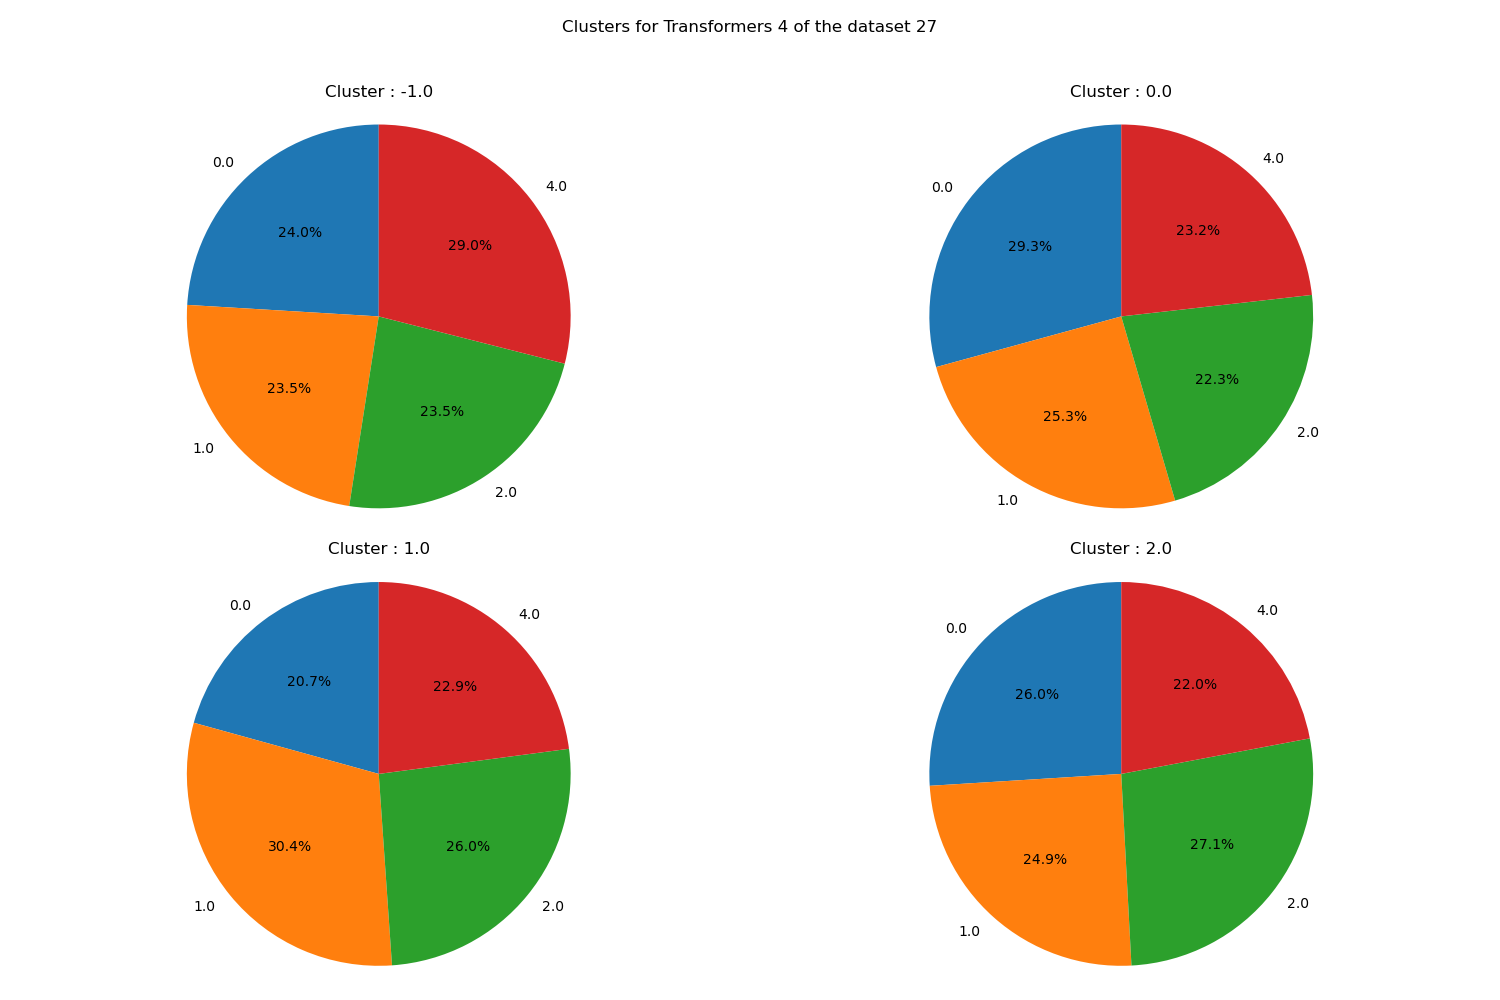
\includegraphics[width=0.8\linewidth]{img/annexes/27/clustering_pie_charts/Transformers 4.png}} \\
\end{longtable}


\begin{longtable}{|c|c|c|c|c|}
\caption{Transformers 6 Clustering Results on 27} \label{tab:27_transformers_6_clustering_results}\\
\hline
\multicolumn{5}{|c|}{\textbf{General Information}} \\
\hline
\multicolumn{2}{|c|}{Min Samples} & \multicolumn{3}{c|}{937} \\
\multicolumn{2}{|c|}{Total Duration} & \multicolumn{3}{c|}{3973.074733 s} \\
\hline
\multicolumn{5}{|c|}{\textbf{Clustering Information}} \\
\hline
EPS & Number of Clusters & Silhouette Score & Noise Points & Duration \\
0.01 & 3 & 0.37613049149513245 & 2636 & 806.924699 s\\
0.02 & 3 & 0.37613049149513245 & 2636 & 759.43715 s\\
0.03 & 3 & 0.37613049149513245 & 2636 & 762.661041 s\\
0.04 & 3 & 0.37613049149513245 & 2636 & 821.687468 s\\
0.05 & 3 & 0.37613049149513245 & 2636 & 818.360119 s\\
\hline
\multicolumn{5}{|c|}{\textbf{Best EPS Information}} \\
\hline
0.01 & 3 & 0.37613049149513245 & 2636 & 806.924699 s\\
\hline
\multicolumn{5}{|c|}{\textbf{Label Association}} \\
\hline
Cluster ID & \multicolumn{2}{c|}{Label} & \multicolumn{2}{c|}{Number of Samples} \\
\hline
\multirow{4}{*}{-1.0} & \multicolumn{2}{c|}{0.0} & \multicolumn{2}{c|}{134} \\
& \multicolumn{2}{c|}{1.0} & \multicolumn{2}{c|}{97} \\
& \multicolumn{2}{c|}{2.0} & \multicolumn{2}{c|}{114} \\
& \multicolumn{2}{c|}{4.0} & \multicolumn{2}{c|}{111} \\
\hline
\multirow{4}{*}{0.0} & \multicolumn{2}{c|}{0.0} & \multicolumn{2}{c|}{81} \\
& \multicolumn{2}{c|}{1.0} & \multicolumn{2}{c|}{86} \\
& \multicolumn{2}{c|}{2.0} & \multicolumn{2}{c|}{53} \\
& \multicolumn{2}{c|}{4.0} & \multicolumn{2}{c|}{72} \\
\hline
\multirow{4}{*}{1.0} & \multicolumn{2}{c|}{0.0} & \multicolumn{2}{c|}{49} \\
& \multicolumn{2}{c|}{1.0} & \multicolumn{2}{c|}{73} \\
& \multicolumn{2}{c|}{2.0} & \multicolumn{2}{c|}{61} \\
& \multicolumn{2}{c|}{4.0} & \multicolumn{2}{c|}{53} \\
\hline
\multirow{4}{*}{2.0} & \multicolumn{2}{c|}{0.0} & \multicolumn{2}{c|}{57} \\
& \multicolumn{2}{c|}{1.0} & \multicolumn{2}{c|}{59} \\
& \multicolumn{2}{c|}{2.0} & \multicolumn{2}{c|}{62} \\
& \multicolumn{2}{c|}{4.0} & \multicolumn{2}{c|}{54} \\
\hline
\multicolumn{5}{|c|}{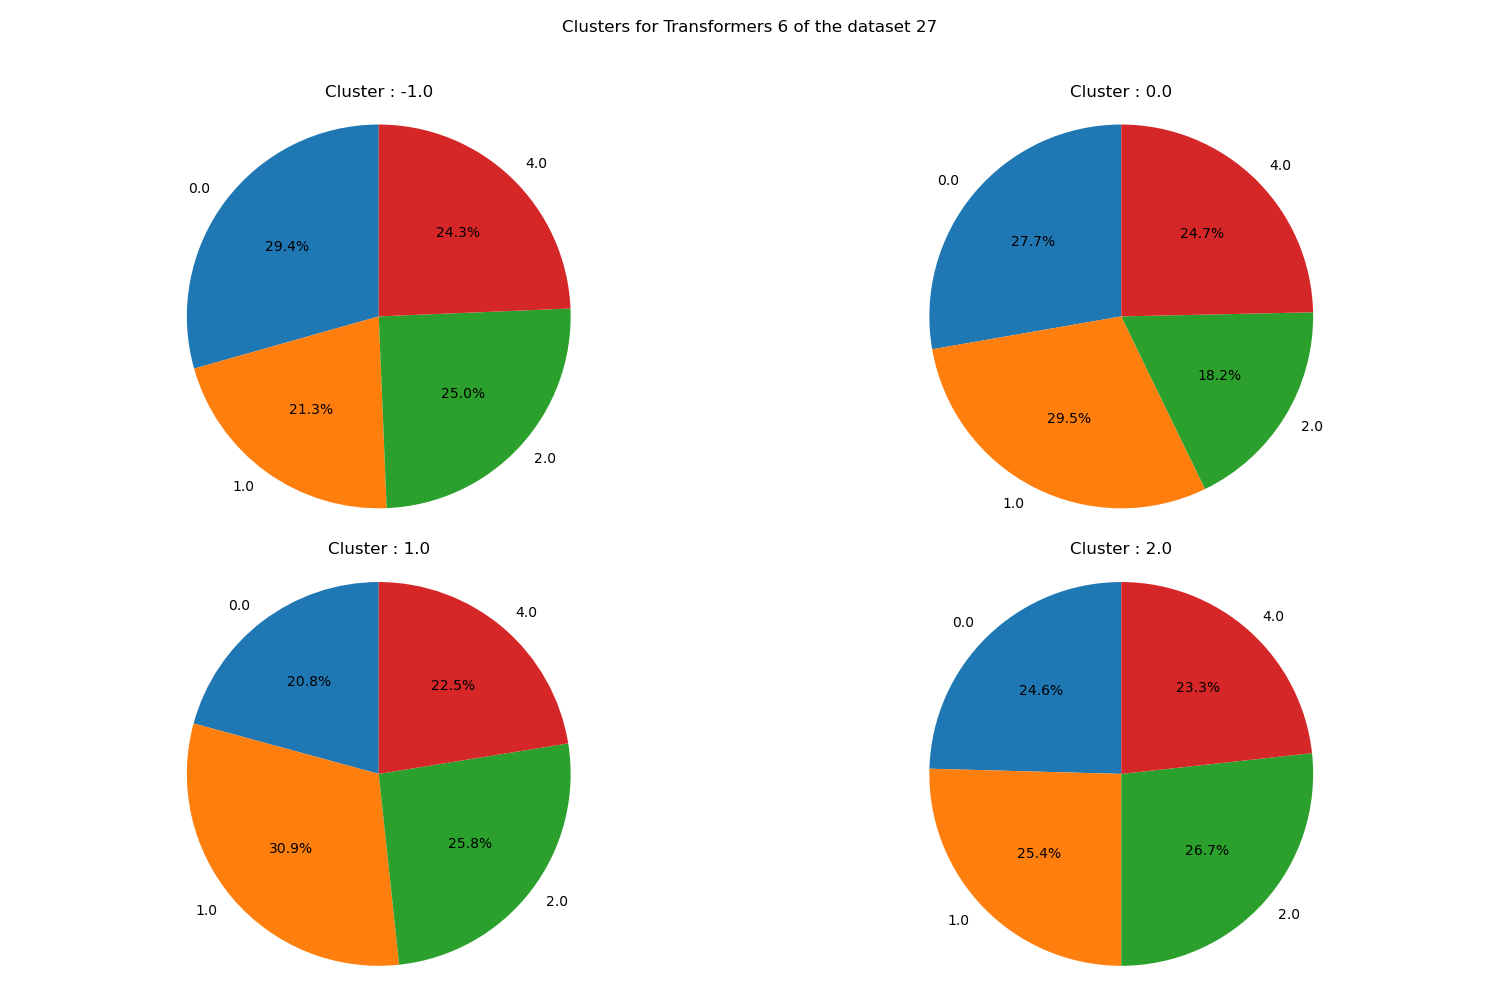
\includegraphics[width=0.8\linewidth]{img/annexes/27/clustering_pie_charts/Transformers 6.png}} \\
\end{longtable}


\begin{longtable}{|c|c|c|c|c|}
\caption{Word2vec 1 Clustering Results on 27} \label{tab:27_word2vec_1_clustering_results}\\
\hline
\multicolumn{5}{|c|}{\textbf{General Information}} \\
\hline
\multicolumn{2}{|c|}{Min Samples} & \multicolumn{3}{c|}{937} \\
\multicolumn{2}{|c|}{Total Duration} & \multicolumn{3}{c|}{4102.458592 s} \\
\hline
\multicolumn{5}{|c|}{\textbf{Clustering Information}} \\
\hline
EPS & Number of Clusters & Silhouette Score & Noise Points & Duration \\
0.01 & 2 & 0.2816171944141388 & 3355 & 861.723101 s\\
0.02 & 2 & 0.24786975979804993 & 3822 & 806.529987 s\\
0.03 & 2 & 0.23544950783252716 & 3938 & 786.201026 s\\
0.04 & 2 & 0.2358776181936264 & 3952 & 838.073615 s\\
0.05 & 2 & 0.2358776181936264 & 3952 & 805.644238 s\\
\hline
\multicolumn{5}{|c|}{\textbf{Best EPS Information}} \\
\hline
0.01 & 2 & 0.2816171944141388 & 3355 & 861.723101 s\\
\hline
\multicolumn{5}{|c|}{\textbf{Label Association}} \\
\hline
Cluster ID & \multicolumn{2}{c|}{Label} & \multicolumn{2}{c|}{Number of Samples} \\
\hline
\multirow{4}{*}{-1.0} & \multicolumn{2}{c|}{0.0} & \multicolumn{2}{c|}{149} \\
& \multicolumn{2}{c|}{1.0} & \multicolumn{2}{c|}{140} \\
& \multicolumn{2}{c|}{2.0} & \multicolumn{2}{c|}{126} \\
& \multicolumn{2}{c|}{4.0} & \multicolumn{2}{c|}{135} \\
\hline
\multirow{4}{*}{0.0} & \multicolumn{2}{c|}{0.0} & \multicolumn{2}{c|}{60} \\
& \multicolumn{2}{c|}{1.0} & \multicolumn{2}{c|}{66} \\
& \multicolumn{2}{c|}{2.0} & \multicolumn{2}{c|}{63} \\
& \multicolumn{2}{c|}{4.0} & \multicolumn{2}{c|}{72} \\
\hline
\multirow{4}{*}{1.0} & \multicolumn{2}{c|}{0.0} & \multicolumn{2}{c|}{112} \\
& \multicolumn{2}{c|}{1.0} & \multicolumn{2}{c|}{109} \\
& \multicolumn{2}{c|}{2.0} & \multicolumn{2}{c|}{101} \\
& \multicolumn{2}{c|}{4.0} & \multicolumn{2}{c|}{83} \\
\hline
\multicolumn{5}{|c|}{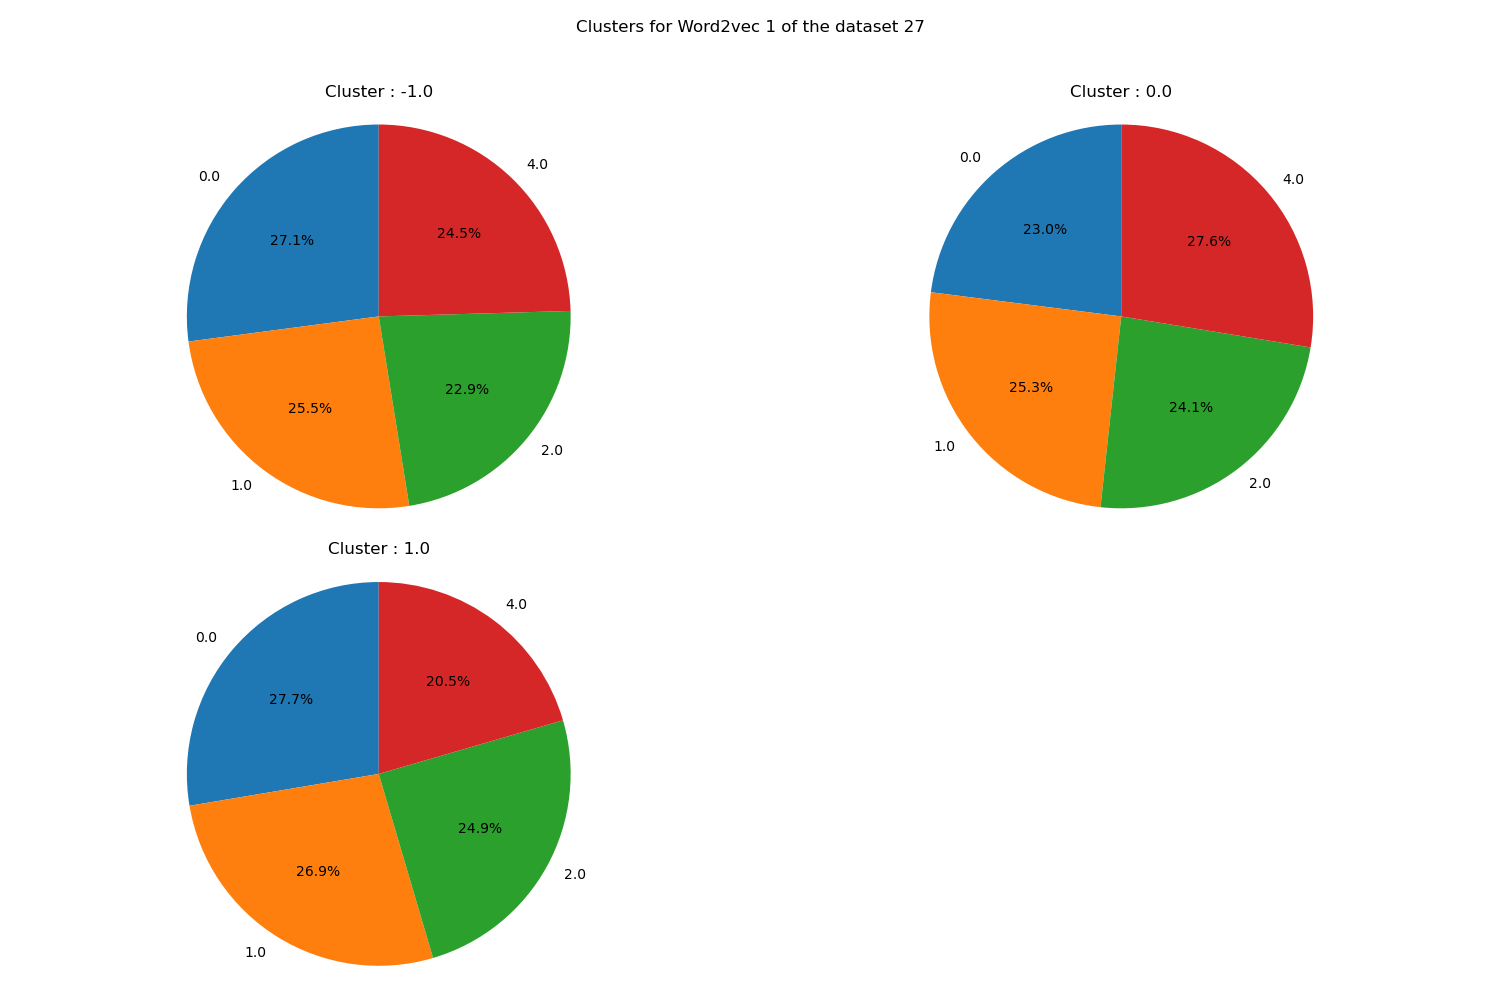
\includegraphics[width=0.8\linewidth]{img/annexes/27/clustering_pie_charts/Word2vec 1.png}} \\
\end{longtable}


\section{Classification results}

\label{sec:annexe:classification_results}

\subsection{26 chunk\_extraction (filtered entropy)}

\begin{figure}[H]
\centering
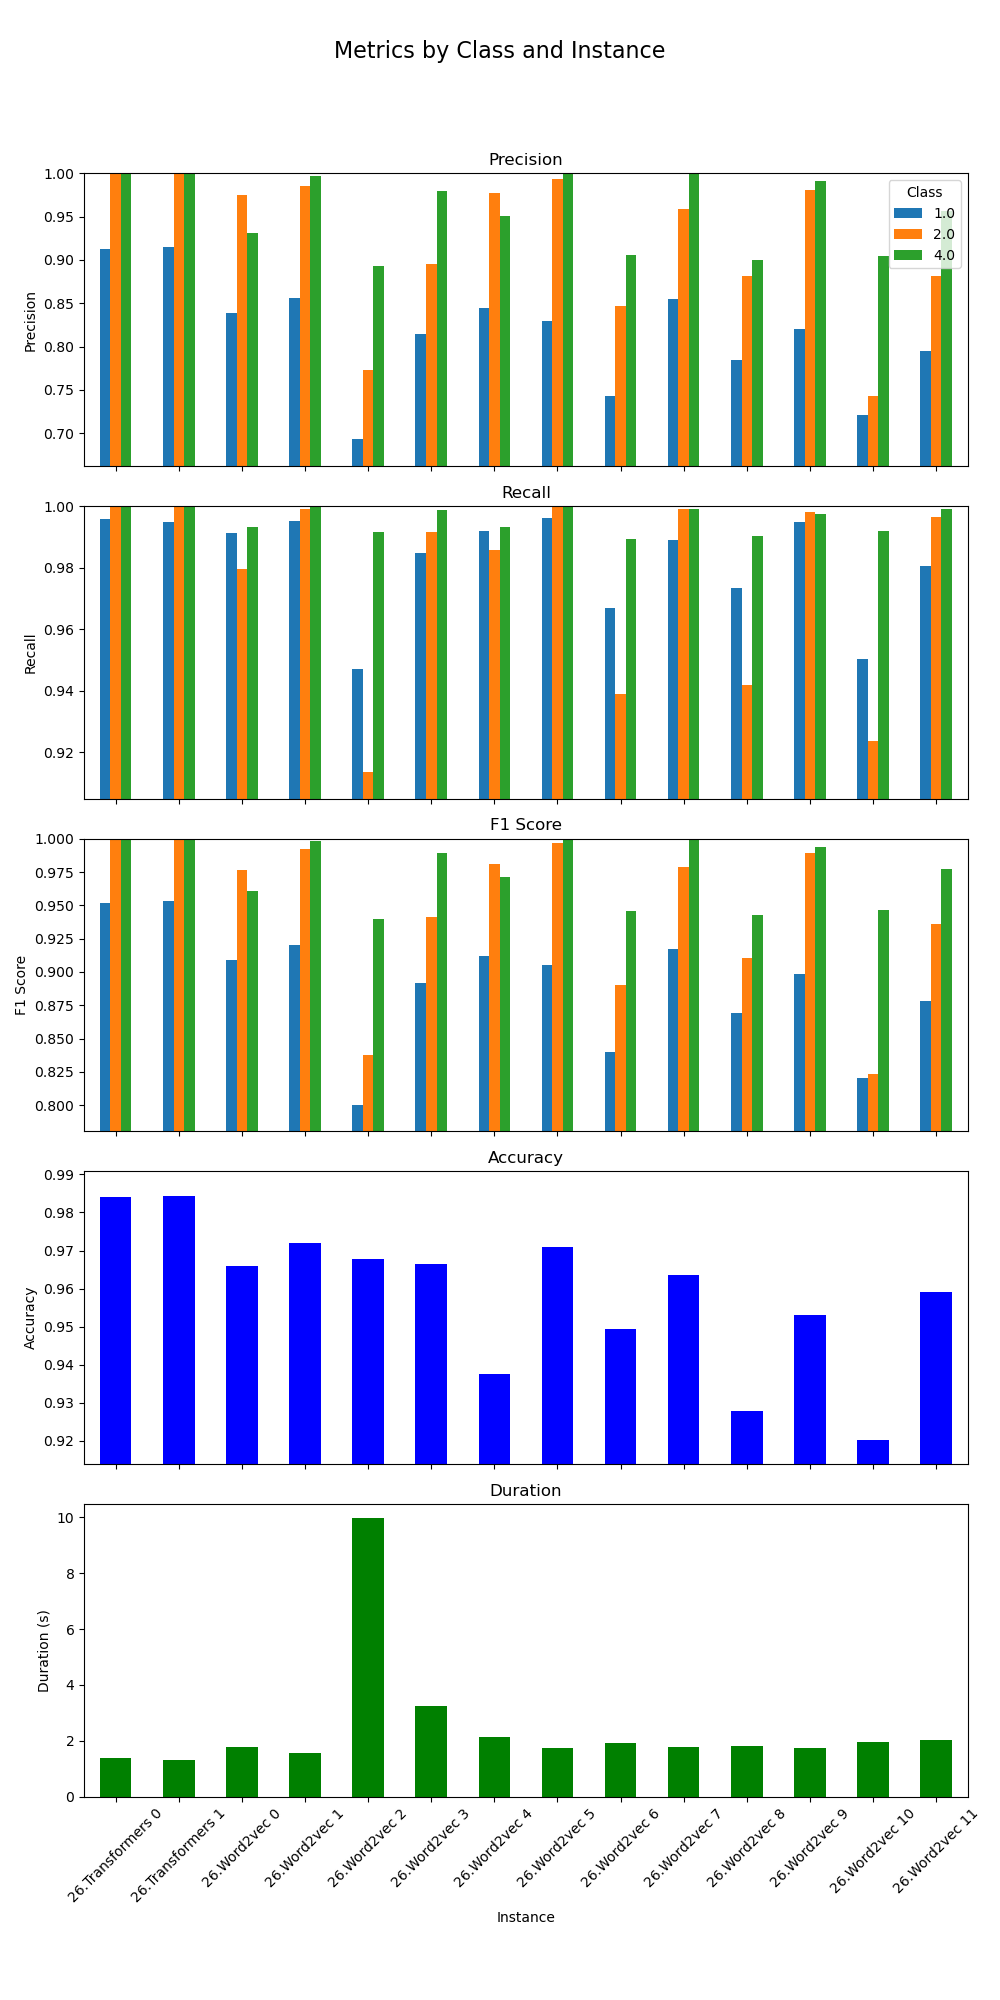
\includegraphics[width=0.6\textwidth]{img/annexes/26/26 - Metrics.png}
\caption{Metrics for the instances of the dataset26}
\label{fig:26_metrics_instance}
\end{figure}

\begin{longtable}{|c|c|c|}
\caption{Transformers 1 Classification Results on 26} \label{tab:26_transformers_1_classifiers_results} \\
\hline
Class & Metric Name & Metric Value \\
\hline
\multirow{4}{*}{0.0} & Precision & 0.9989467459994826 \\
 & Recall & 0.9811611825985953 \\
 & F1 Score & 0.9899740882829596 \\
 & Support & 110198.0 \\
 & Final Samples (after rebalancing) & 20964 \\
 & Initial Samples (before rebalancing) & 620669 \\
\hline
\multirow{4}{*}{1.0} & Precision & 0.9148202855736091 \\
 & Recall & 0.9949129852744311 \\
 & F1 Score & 0.953187123252533 \\
 & Support & 22410.0 \\
 & Final Samples (after rebalancing) & 20964 \\
 & Initial Samples (before rebalancing) & 125784 \\
\hline
\multirow{4}{*}{2.0} & Precision & 1.0 \\
 & Recall & 1.0 \\
 & F1 Score & 1.0 \\
 & Support & 3735.0 \\
 & Final Samples (after rebalancing) & 20964 \\
 & Initial Samples (before rebalancing) & 20964 \\
\hline
\multirow{4}{*}{4.0} & Precision & 1.0 \\
 & Recall & 1.0 \\
 & F1 Score & 1.0 \\
 & Support & 3735.0 \\
 & Final Samples (after rebalancing) & 20964 \\
 & Initial Samples (before rebalancing) & 20964 \\
\hline
\multirow{4}{*}{Macro Avg} & Precision & 0.9784417578932729 \\
 & Recall & 0.9940185419682566 \\
 & F1 Score & 0.9857903028838731 \\
 & Support & 140078.0 \\
 & Final Samples (after rebalancing) & 83856 \\
 & Initial Samples (before rebalancing) & 788381 \\
\hline
\multirow{4}{*}{Weighted Avg} & Precision & 0.985544169072628 \\
 & Recall & 0.9843658533102986 \\
 & F1 Score & 0.9846234812939566 \\
 & Support & 140078.0 \\
 & Final Samples (after rebalancing) & 83856 \\
 & Initial Samples (before rebalancing) & 788381 \\
\hline
& Accuracy & 0.9843658533102986 \\ \hline
& True Positives & 22296 \\ \hline
& True Negatives & 108122 \\ \hline
& False Positives & 2076 \\ \hline
& False Negatives & 114 \\ \hline
& AUC & 0.93 \\ \hline
& Duration (seconds) & 1.309276 \\ \hline
\end{longtable}


\begin{longtable}{|c|c|c|}
\caption{Word2vec 1 Classification Results on 26} \label{tab:26_word2vec_1_classifiers_results} \\
\hline
Class & Metric Name & Metric Value \\
\hline
\multirow{4}{*}{0.0} & Precision & 0.9991360772271836 \\
 & Recall & 0.9655256901214178 \\
 & F1 Score & 0.9820433893737107 \\
 & Support & 110198.0 \\
 & Final Samples (after rebalancing) & 20964 \\
 & Initial Samples (before rebalancing) & 620669 \\
\hline
\multirow{4}{*}{1.0} & Precision & 0.8559530206494205 \\
 & Recall & 0.9951360999553771 \\
 & F1 Score & 0.9203119841531859 \\
 & Support & 22410.0 \\
 & Final Samples (after rebalancing) & 20964 \\
 & Initial Samples (before rebalancing) & 125784 \\
\hline
\multirow{4}{*}{2.0} & Precision & 0.9854766305782942 \\
 & Recall & 0.9991967871485944 \\
 & F1 Score & 0.9922892847646901 \\
 & Support & 3735.0 \\
 & Final Samples (after rebalancing) & 20964 \\
 & Initial Samples (before rebalancing) & 20964 \\
\hline
\multirow{4}{*}{4.0} & Precision & 0.9970635344367326 \\
 & Recall & 1.0 \\
 & F1 Score & 0.9985296083411309 \\
 & Support & 3735.0 \\
 & Final Samples (after rebalancing) & 20964 \\
 & Initial Samples (before rebalancing) & 20964 \\
\hline
\multirow{4}{*}{Macro Avg} & Precision & 0.9594073157229077 \\
 & Recall & 0.9899646443063473 \\
 & F1 Score & 0.9732935666581793 \\
 & Support & 140078.0 \\
 & Final Samples (after rebalancing) & 83856 \\
 & Initial Samples (before rebalancing) & 788381 \\
\hline
\multirow{4}{*}{Weighted Avg} & Precision & 0.9758098498505534 \\
 & Recall & 0.972079841231314 \\
 & F1 Score & 0.972880234960717 \\
 & Support & 140078.0 \\
 & Final Samples (after rebalancing) & 83856 \\
 & Initial Samples (before rebalancing) & 788381 \\
\hline
& Accuracy & 0.972079841231314 \\ \hline
& True Positives & 22301 \\ \hline
& True Negatives & 106399 \\ \hline
& False Positives & 3750 \\ \hline
& False Negatives & 92 \\ \hline
& AUC & 0.92 \\ \hline
& Duration (seconds) & 1.557051 \\ \hline
\end{longtable}


\subsection{24 chunk\_extraction}

\subsection{25 chunk\_extraction (filtered chunk size)}

\begin{figure}[H]
\centering
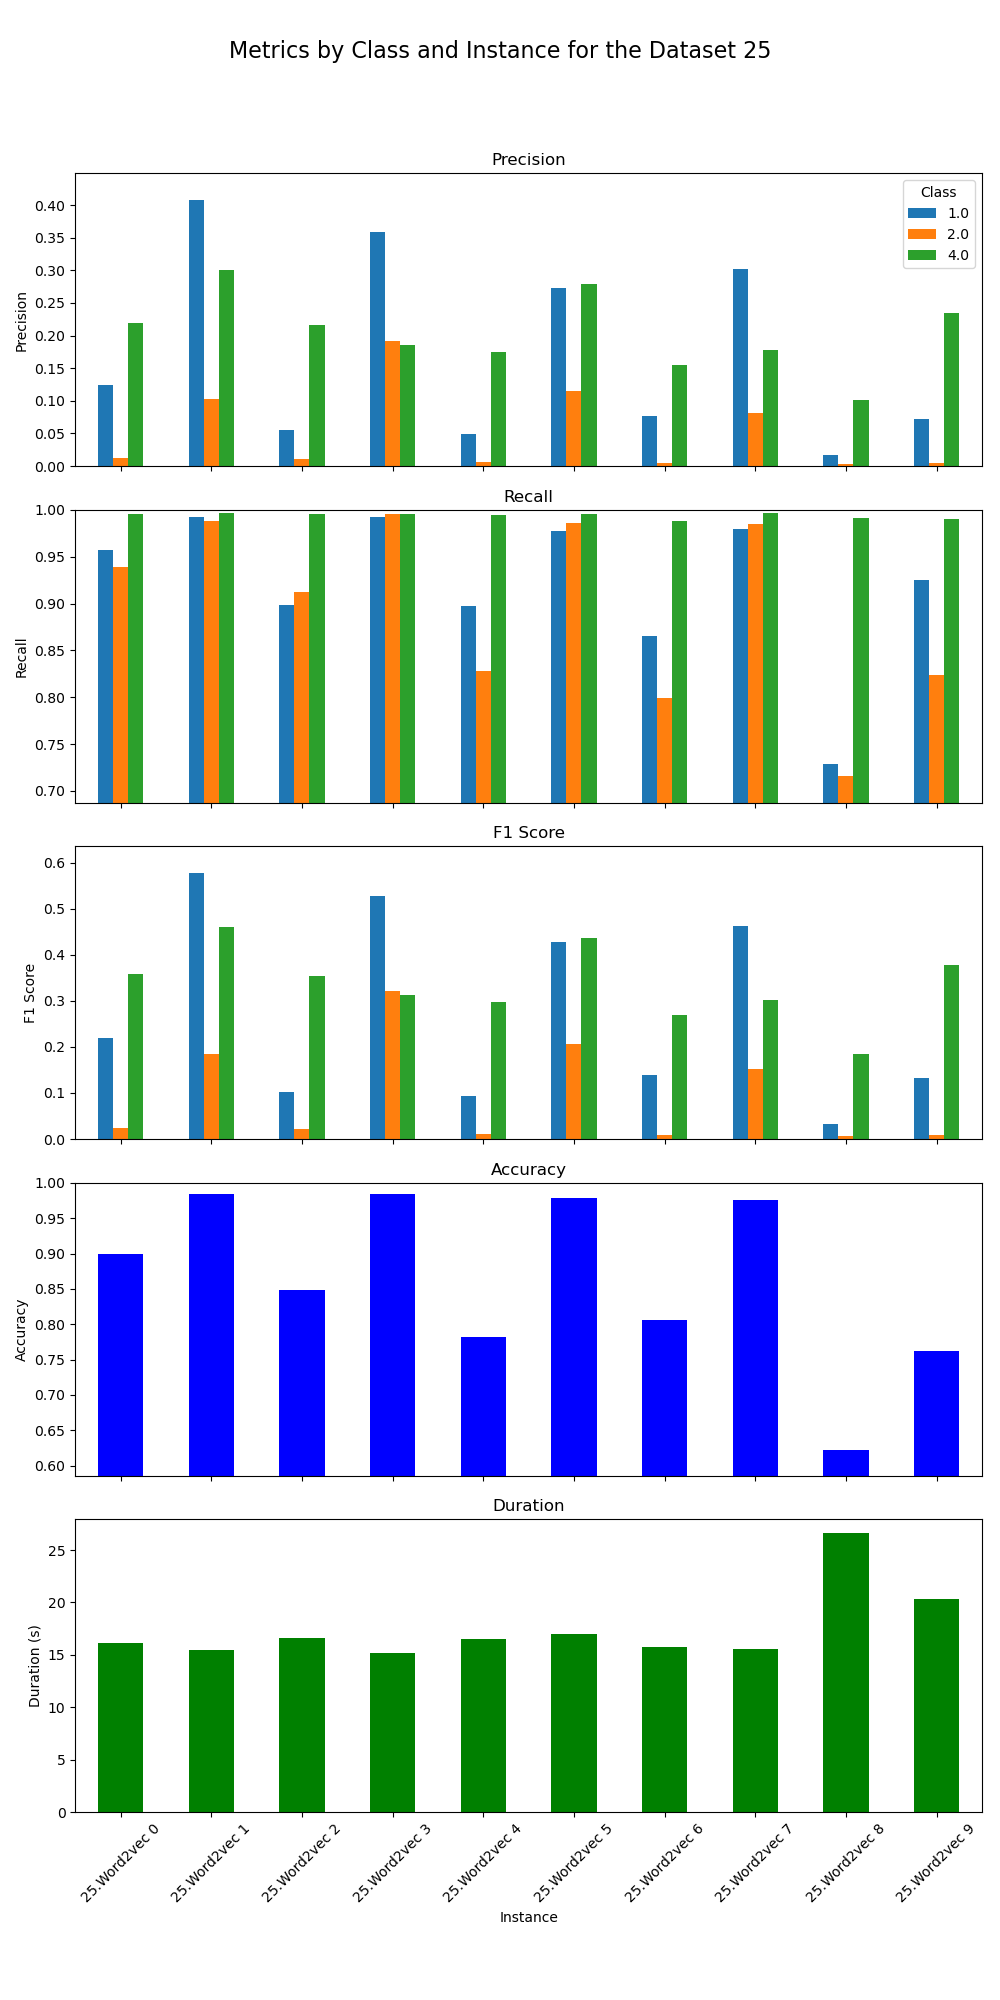
\includegraphics[width=0.6\textwidth]{img/annexes/25/25 - Metrics.png}
\caption{Metrics for the instances of the dataset25}
\label{fig:25_metrics_instance}
\end{figure}

\begin{longtable}{|c|c|c|}
\caption{Word2vec 3 Classification Results on 25} \label{tab:25_word2vec_3_classifiers_results} \\
\hline
Class & Metric Name & Metric Value \\
\hline
\multirow{4}{*}{0.0} & Precision & 0.9999617471431186 \\
 & Recall & 0.9838132974079551 \\
 & F1 Score & 0.9918217959650952 \\
 & Support & 4437346.0 \\
 & Final Samples (after rebalancing) & 20964 \\
 & Initial Samples (before rebalancing) & 24506437 \\
\hline
\multirow{4}{*}{1.0} & Precision & 0.35848600570406536 \\
 & Recall & 0.9927710843373494 \\
 & F1 Score & 0.5267606634229499 \\
 & Support & 22410.0 \\
 & Final Samples (after rebalancing) & 20964 \\
 & Initial Samples (before rebalancing) & 125784 \\
\hline
\multirow{4}{*}{2.0} & Precision & 0.19214470284237725 \\
 & Recall & 0.9954484605087015 \\
 & F1 Score & 0.32211392679228934 \\
 & Support & 3735.0 \\
 & Final Samples (after rebalancing) & 20964 \\
 & Initial Samples (before rebalancing) & 20964 \\
\hline
\multirow{4}{*}{4.0} & Precision & 0.18481717011128776 \\
 & Recall & 0.9959839357429718 \\
 & F1 Score & 0.31177974269790054 \\
 & Support & 3735.0 \\
 & Final Samples (after rebalancing) & 20964 \\
 & Initial Samples (before rebalancing) & 20964 \\
\hline
\multirow{4}{*}{Macro Avg} & Precision & 0.4338524064502122 \\
 & Recall & 0.9920041944992445 \\
 & F1 Score & 0.5381190322195588 \\
 & Support & 4467226.0 \\
 & Final Samples (after rebalancing) & 83856 \\
 & Initial Samples (before rebalancing) & 24674149 \\
\hline
\multirow{4}{*}{Weighted Avg} & Precision & 0.9953868201030884 \\
 & Recall & 0.9838781382450765 \\
 & F1 Score & 0.9883602885462669 \\
 & Support & 4467226.0 \\
 & Final Samples (after rebalancing) & 83856 \\
 & Initial Samples (before rebalancing) & 24674149 \\
\hline
& Accuracy & 0.9838781382450765 \\ \hline
& True Positives & 22248 \\ \hline
& True Negatives & 4365520 \\ \hline
& False Positives & 39808 \\ \hline
& False Negatives & 140 \\ \hline
& AUC & 0.98 \\ \hline
& Duration (seconds) & 15.149247 \\ \hline
\end{longtable}


\subsection{27 chunk\_extraction (filtered entropy and chunk size)}

\begin{figure}[H]
\centering
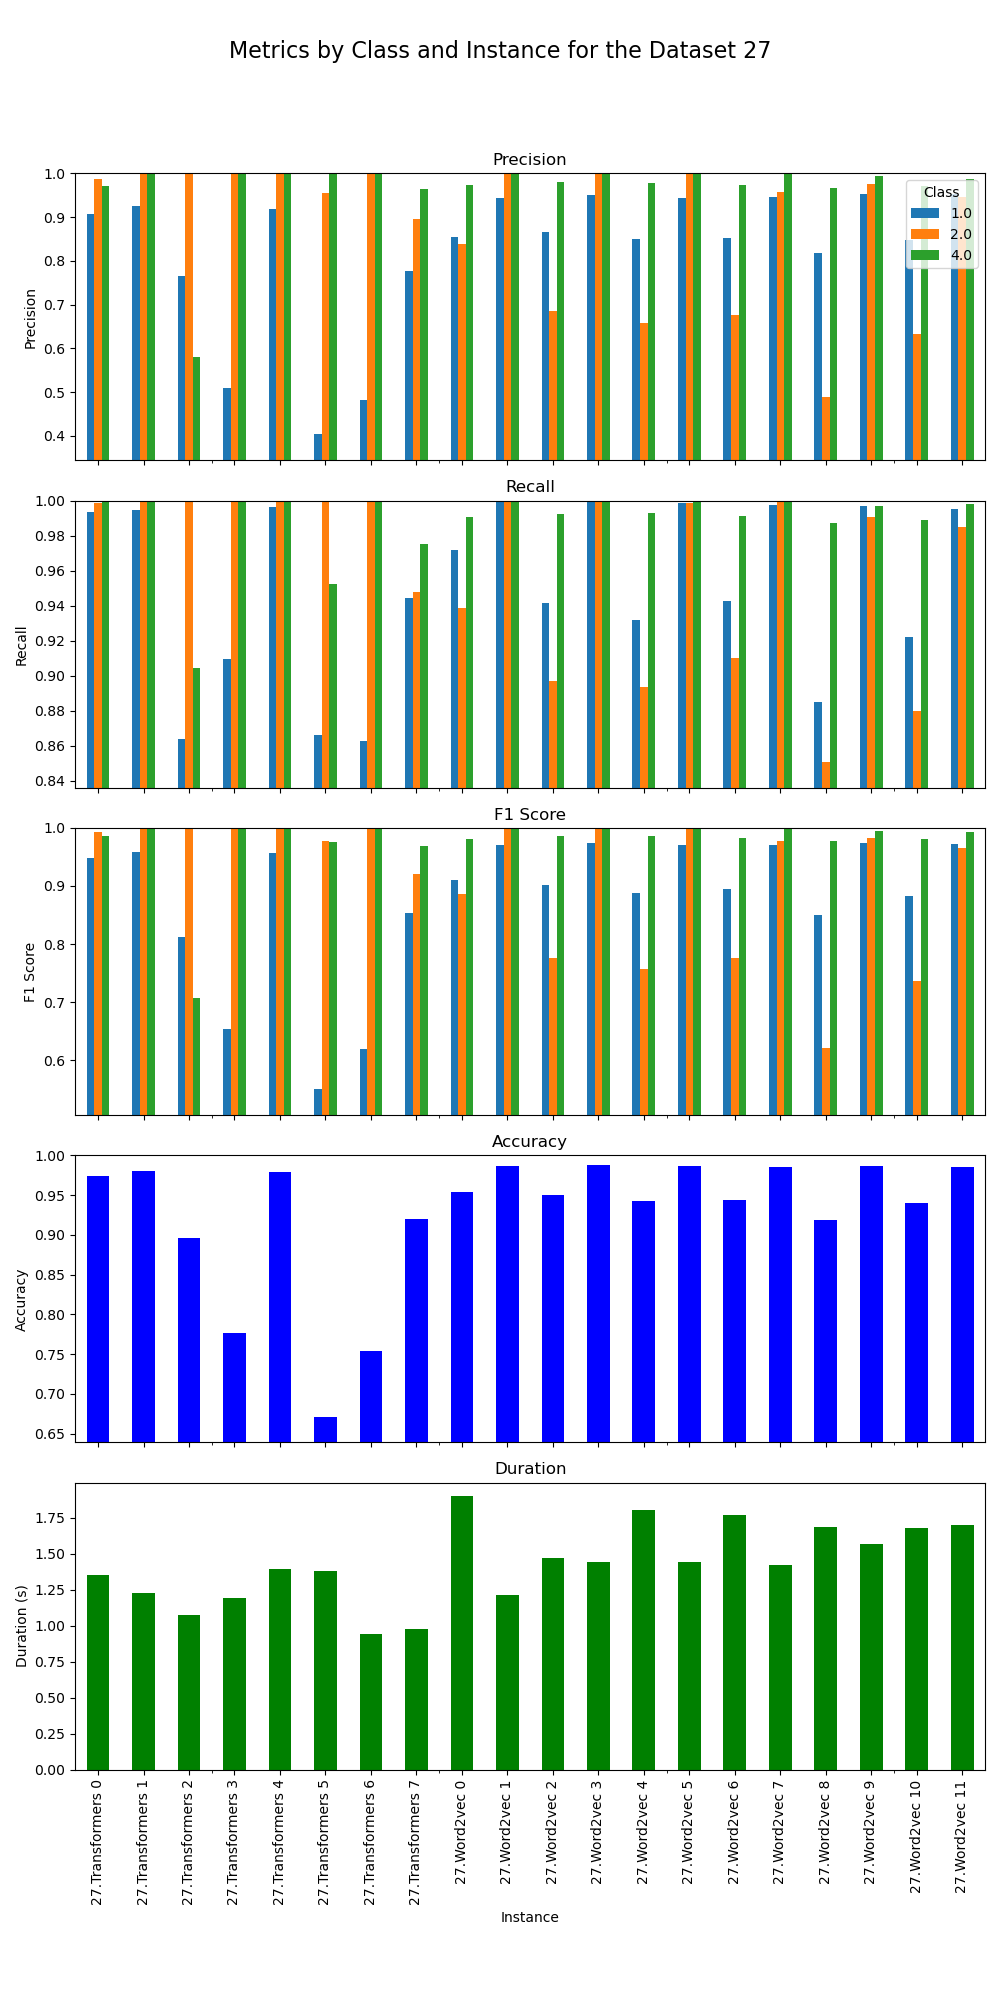
\includegraphics[width=0.6\textwidth]{img/annexes/27/27 - Metrics.png}
\caption{Metrics for the instances of the dataset27}
\label{fig:27_metrics_instance}
\end{figure}

\begin{longtable}{|c|c|c|}
\caption{Transformers 1 Classification Results on 27} \label{tab:27_transformers_1_classifiers_results} \\
\hline
Class & Metric Name & Metric Value \\
\hline
\multirow{4}{*}{0.0} & Precision & 0.9981469570277803 \\
 & Recall & 0.9728055642621531 \\
 & F1 Score & 0.9853133479973091 \\
 & Support & 66999.0 \\
 & Final Samples (after rebalancing) & 20964 \\
 & Initial Samples (before rebalancing) & 376160 \\
\hline
\multirow{4}{*}{1.0} & Precision & 0.9244328314877027 \\
 & Recall & 0.9946006247211067 \\
 & F1 Score & 0.958233915865953 \\
 & Support & 22410.0 \\
 & Final Samples (after rebalancing) & 20964 \\
 & Initial Samples (before rebalancing) & 125784 \\
\hline
\multirow{4}{*}{2.0} & Precision & 0.9997323340471093 \\
 & Recall & 1.0 \\
 & F1 Score & 0.9998661491098916 \\
 & Support & 3735.0 \\
 & Final Samples (after rebalancing) & 20964 \\
 & Initial Samples (before rebalancing) & 20964 \\
\hline
\multirow{4}{*}{4.0} & Precision & 1.0 \\
 & Recall & 0.9997322623828648 \\
 & F1 Score & 0.9998661132681751 \\
 & Support & 3735.0 \\
 & Final Samples (after rebalancing) & 20964 \\
 & Initial Samples (before rebalancing) & 20964 \\
\hline
\multirow{4}{*}{Macro Avg} & Precision & 0.9805780306406481 \\
 & Recall & 0.9917846128415311 \\
 & F1 Score & 0.9858198815603322 \\
 & Support & 96879.0 \\
 & Final Samples (after rebalancing) & 83856 \\
 & Initial Samples (before rebalancing) & 543872 \\
\hline
\multirow{4}{*}{Weighted Avg} & Precision & 0.9812280060199797 \\
 & Recall & 0.9799337317684947 \\
 & F1 Score & 0.9801714618958681 \\
 & Support & 96879.0 \\
 & Final Samples (after rebalancing) & 83856 \\
 & Initial Samples (before rebalancing) & 543872 \\
\hline
& Accuracy & 0.9799337317684947 \\ \hline
& True Positives & 22289 \\ \hline
& True Negatives & 65177 \\ \hline
& False Positives & 1822 \\ \hline
& False Negatives & 121 \\ \hline
& AUC & 0.89 \\ \hline
& Duration (seconds) & 1.23036 \\ \hline
\end{longtable}


\begin{longtable}{|c|c|c|}
\caption{Word2vec 3 Classification Results on 27} \label{tab:27_word2vec_3_classifiers_results} \\
\hline
Class & Metric Name & Metric Value \\
\hline
\multirow{4}{*}{0.0} & Precision & 0.9997874343323919 \\
 & Recall & 0.9828206391140166 \\
 & F1 Score & 0.9912314373668721 \\
 & Support & 66999.0 \\
 & Final Samples (after rebalancing) & 20964 \\
 & Initial Samples (before rebalancing) & 376160 \\
\hline
\multirow{4}{*}{1.0} & Precision & 0.9511148863877681 \\
 & Recall & 0.9992860330209727 \\
 & F1 Score & 0.9746055924273745 \\
 & Support & 22410.0 \\
 & Final Samples (after rebalancing) & 20964 \\
 & Initial Samples (before rebalancing) & 125784 \\
\hline
\multirow{4}{*}{2.0} & Precision & 0.9991972170189992 \\
 & Recall & 0.9997322623828648 \\
 & F1 Score & 0.9994646680942185 \\
 & Support & 3735.0 \\
 & Final Samples (after rebalancing) & 20964 \\
 & Initial Samples (before rebalancing) & 20964 \\
\hline
\multirow{4}{*}{4.0} & Precision & 1.0 \\
 & Recall & 1.0 \\
 & F1 Score & 1.0 \\
 & Support & 3735.0 \\
 & Final Samples (after rebalancing) & 20964 \\
 & Initial Samples (before rebalancing) & 20964 \\
\hline
\multirow{4}{*}{Macro Avg} & Precision & 0.9875248844347898 \\
 & Recall & 0.9954597336294635 \\
 & F1 Score & 0.9913254244721164 \\
 & Support & 96879.0 \\
 & Final Samples (after rebalancing) & 83856 \\
 & Initial Samples (before rebalancing) & 543872 \\
\hline
\multirow{4}{*}{Weighted Avg} & Precision & 0.9885139661056759 \\
 & Recall & 0.9879437236139927 \\
 & F1 Score & 0.9880410298802881 \\
 & Support & 96879.0 \\
 & Final Samples (after rebalancing) & 83856 \\
 & Initial Samples (before rebalancing) & 543872 \\
\hline
& Accuracy & 0.9879437236139927 \\ \hline
& True Positives & 22394 \\ \hline
& True Negatives & 65848 \\ \hline
& False Positives & 1150 \\ \hline
& False Negatives & 14 \\ \hline
& AUC & 0.89 \\ \hline
& Duration (seconds) & 1.442202 \\ \hline
\end{longtable}


